%$Id: thesis-e.tex,v 1.4 2003/01/20 06:05:12 gondow Exp $
\documentclass[12pt]{report}
\usepackage{jaist-e-master}
\usepackage{llncsdoc}
% *** MISC UTILITY PACKAGES ***
%
\newtheorem{definition}{Definition}
\newtheorem{theorem}{Theorem}
\newtheorem{proof}{Proof}
\newtheorem{example}{Example}
\newtheorem{lemma}{Lemma}
\usepackage{amssymb}
\setcounter{tocdepth}{3}

\usepackage{graphicx}
\graphicspath{ {Figs/} }

\usepackage{amsmath}
\usepackage{multirow}
\usepackage{slashbox}
\usepackage{amsfonts}

\usepackage{algorithm2e}
\usepackage{epstopdf}
\usepackage{array}
\usepackage{enumerate}

\usepackage{epstopdf}

\usepackage{url}
%\urldef{\mailsa}\path|{khanhtv, mizuhito}@jaist.ac.jp|    

%ieee requirements
%\usepackage[utf8]{inputenc}
%\usepackage[T1]{fontenc}
%\usepackage{microtype} 
%\usepackage{balance}

%user definitions
\newcommand{\Nat}{{\mathbb N}}
\newcommand{\Real}{{\mathbb R}}
\newcommand{\Rat}{{\mathbb Q}}
\newcommand{\suppress}[1]{} % Comment out text.
\newcommand{\mizuhito}[1]{\{{\bf Mizuhito:~\sf #1}\}} % Highlight text.
\newcommand{\khanh}[1]{\{{\bf Khanh:~\sf #1}\}} % Highlight text.

\newcommand{\smallHead}[1]{%
    \par\vspace{.35cm}\noindent\textbf{#1}%
    \par\noindent\ignorespaces%
}

\newcommand\TTTT{%
 \textsf{T\kern-0.2em\raisebox{-0.3em}T\kern-0.2emT\kern-0.2em\raisebox{-0.3em}2}%
}

% correct bad hyphenation here
\hyphenation{op-tical net-works semi-conduc-tor}
%
\title{Equality handling and efficiency improvement of SMT for non-linear constraints over reals}                                %% title 
\author{VU XUAN TUNG}{1310007}                %% author's name
\school{Information Science}                 %% school
\adviser{Professor Mizuhito Ogawa}   %% your adviser
\judge{Associate Professor Satoshi Sato}     %% chief judge
      {Professor Takuya Katayama}            %% judge 
      {Associate Professor Katsuhiko Gondow} %% judge
\date{February, 2003}{March, 2003}
   %% submitted date (month, year), graduated date (month, year)

\begin{document}
\maketitle

\begin{abstract}
This thesis presents an SMT solver {\bf raSAT} for polynomial constraints. Solving polynomial constraints is raised from many applications of Software verification such as roundoff/overflow error analysis, automatic termination proving or loop invariant generation. In 1948, Tarski proposed a decision method for solving polynomial constraints over real numbers.  
{\bf raSAT} consists of a simple iterative approximation refinement, called {\bf raSAT} loop, 
which is an extension of the standard ICP (Interval Constraint Propagation) with testing. 
Two approximation schemes consist of interval arithmetic (over-approximation) and 
testing (under-approximation), to accelerate SAT detection. 
If both fails, input intervals are refined by decomposition. 

ICP is robust for large degrees, but the number of boxes (products of intervals) to explore 
exponentially explodes when the number of variables increases. 
We design strategies for boosting SAT detection on the choice of a variable to decompose
and a box to explore. 

to choose a variable for decomposition and a box by 
targeting on SAT detection. 

Several heuristic measures, called {\em SAT likelyhood}, {\em sensitivity}, and the number of 
unsolved atomic polynomial constraints, are compared on Zankl and Meti-Tarski benchmarks from 
QF\_NRA category of SMT-LIB. They are also evaluated by comparing {\bf Z3 4.3} and {\bf iSAT3}. 
We also show a simple modification to handle mixed intergers, and experiments on 
AProVE benchmark from QF\_NIA category of SMT-LIB.
\end{abstract}

\chapter{Introduction}
\section{Polynomial constraint solving}
{\em Polynomial constraint solving} is a task of computing an assignment of variables to real/integer numbers 
that satisfies given polynomial inequalities/equations. If such an assignment exists, the constraint is said to be satisfiable (SAT) and the assignment is called SAT instance; otherwise we mention it as unsatisfiable (UNSAT). 
\begin{example} \label{examp:unsat-example}
$x^2 + y^2 < 1 \wedge xy > 1$ is an example of an UNSAT constraint. While the set of satisfiable points for the first inequality ($x^2 + y^2 < 1$) is the read circle in Figure \ref{fig:unsat-example}, the set for the second one is the green area. Because these two areas do not intersect, the conjunction of two equalities is UNSAT.
\end{example}

\begin{figure}[ht]
%\begin{minipage}[b]{1.0\linewidth}
\centering
\includegraphics{UNSAT-example.png} 
\caption{Example of UNSAT constraint} 
\label{fig:unsat-example} 
%\end{minipage}
\end{figure} 

\begin{example} \label{examp:sat-example}
Figure~\ref{fig:sat-example} illustrates the satisfiability of the constraint: $x^2 + y^2 < 4 \wedge xy > 1$. Any point in the purple area is a SAT instance of the constraint, e.g. $(1.5, 1)$.
\end{example}

\begin{figure}[ht]
%\begin{minipage}[b]{1.0\linewidth}
\centering
\includegraphics{SAT-example.png} 
\caption{Example of SAT constraint} 
\label{fig:sat-example} 
%\end{minipage}
\end{figure} 

%For instance, $\exists x y. -y^2 + (x^2 - 1) y - 1 > 0 \wedge -x^2 - y^2 + 4 > 0$ is 
%such an example. This is an easy formula, but proving its satisfiability and 
%showing a satisfiable instance (e.g., $x = 1.8$, $y=0.9$) are not so easy.  
%its satisfiability and a satisfiable instance 
%(e.g., $x = 1.8$, $y=0.9$) are not so easy.  		
%
Solving polynomial constraints has many application in Software Verification, such as 
\begin{itemize}
\item {\bf Locating roundoff and overflow errors}, 
which is our motivation~\cite{Ngoc:2009:ORE:1685167.1685421,Ngoc:2010:CRE:1858996.1859056}
%DSP decorders in practice are defined by reference algorithms in C using floating point arithmetic. 
%In embedded systems, often it is replaced with fixed point arithmetic, 
%which may cause visible noises. 
%and locating such roundoff error source is not easy. 
%For instance, consider DSP decoder like mpeg4. Usually, the decoder definition is given by a reference 
%algorithm in C, which uses floating point number. 
%In an embedded system, it is tempting to replace floating 
%point into fixed point numbers. However, naive replacement would cause 

\item {\bf Automatic termination proving}, 
which reduces termination detection to finding a suitable ordering~\cite{Lucas:2008:CCS:1361735.1361760}, 
e.g., \TTTT~\footnote{\url{http://cl-informatik.uibk.ac.at/software/ttt2/}}, 
Aprove~\footnote{\url{http://aprove.informatik.rwth-aachen.de}}. 
%as a solution of polynomial constraints. 

\item {\bf Loop invariant generation}. 
Farkas's lemma is a popular approach in linear loop invariant generation~\cite{Colon}, 
and is reduced to degree $2$ polynomials. 
%matrix multiplications. 
%degree $2$ polynomial constraints. 
%Farkas's lemma uses products of matrices, and it requires solving polynomial constraints of degree 2.
Non-linear loop invariant~\cite{Sankaranarayanan:2004:NLI:982962.964028} requires more complex polynomials.

\item {\bf Hybrid system}. SMT for QF\_NRA are often used as backend engines~\cite{Sankaranarayanan04constructinginvariants}. 

\item {\bf Mechanical contrnol design}. 
PID control is simple but widely used, and designing parameters is 
reduced to polynomial constraints~\cite{control}. 
%Fujitsu used polynomial constraints solving to design PID control of HDD head movement
\end{itemize}	

\section{Existing approaches}
Although solving polynomial constraints on real numbers is decidable~\cite{tarski}, current methodologies have their own pros and cos. They can be classified into the following categories: 
\begin{enumerate}
\item \textbf{Quantifier elimination by cylindrical algebraic decomposition (QE-CAD)} ~\cite{qecad} 
is a complete technique, and 
is implemented in Mathematica, Maple/SynRac, Reduce/Redlog, QEPCAD-B, and recently 
in
Z3 4.3 (which is referred as nlsat in~\cite{Jovanovic13}).
Although QE-CAD is precise and detects beyond SAT instances (e.g., SAT regions), 
scalability is still challenging, since it is DEXPTIME. 
%Since QE-CAD is DEXPTIME wrt the number of variables, 

\item \textbf{Virtual substitution (VS)}. ~
SMT-RAT toolbox \cite{smtrat}\cite{vssmt} combines 
VS, incremental DPLL, and %less lazy and 
eager theory propagation. 
Z3 (version 3.1), the winner of QF\_NRA in SMT competition 2011, 
combines VS, ICP, and linearization.

\item \textbf{Bit-blasting}. ~Bit-blasting in bounded bit width is often used in SMTs for QF\_NIA. 
UCLID~\cite{uclid} reduces the number of bits (i.e., narrowing bounds for SAT instances) 
as an under-approximation, and removes clauses as an over-approximation. 
They refine each other, which shares a similar sprit with {\bf raSAT} loop. 
MiniSmt~\cite{minismt}, the winner of QF\_NRA in SMT competition 2010, 
applies it for rational numbers with symbolic representations for prefixed algebraic numbers. 
MiniSmt can show SAT quickly with small degree polynomials, but due to the bounded bit encoding, 
it cannot conclude UNSAT.
Bit-blasting also suffers a lot when the degree of polynomials increases. 

\item \textbf{Linearization}. ~
CORD \cite{cord} uses another linearization, called 
CORDIC (COrdinate Rotation DIgital Computer) for real numbers. 
Both Barcelogic and CORD apply Yices for solving linear constraints.
Linearization also suffers a lot when the degree of polynomials increases. 

\item \textbf{Interval Constraint Propagation} 
which are used in SMT solver community, e.g., {\bf iSAT3}~\cite{isat}, 
{\bf dReal}~\cite{dRealCADE13}, and RSOLVER~\cite{rsolver}. 
ICP is based on over-approximation by interval arithmetics, and iteratively refines by
interval decompositions. 
It is practically often more efficient than algebraic computation 
with weaker theoretical completeness. 
\end{enumerate}

\section{Proposed Approach and Contributions}
Our aim is an SMT solver for solving polynomial constraint. We first focus on strict inequalities because of the following reasons.
\begin{enumerate}
\item
Satisfiable inequalities allow over-approximation. An over-approximation estimates the range of a polynomial $f$ as $O.range(f)$ that covers all the possible values of $f$, i.e. $range(f) \subseteq O.range(f)$. For an inequality $f>0$, if $O.range(f)$ stays in the positive side, it can be concluded as SAT. On the other hand, over-approximation cannot prove the satisfiability of SAT equations.
\item
Satisfiable inequalities allow under-approximation. An under-approximation computes the range of the polynomial $f$ as  $U.range(f)$ such that $range(f) \supseteq U.range(f)$. If $U.range(f)$ is on the positive side, $f > 0$ can be said to be SAT. Due to the continuity of $f$, finding such an under-approximation for solving $f > 0$ is more feasible than that for $f = 0$.
\begin{itemize}
\item If $f(\bar{x}) > 0$ has a real solution $\bar{x_0}$, there exist rational points near $\bar{x_0}$ which also satisfy the inequality. Solving inequalities over real numbers thus can be reduced to that over rational numbers.
\item The real solution of $f(\bar{x}) = 0$ cannot be approximated to any rational number.
\end{itemize}
\end{enumerate}
For UNSAT constraint (both inequalities and equations) can be solved by over-approximation. Suppose $O.range(f)$ is the result of an over-approximation for a polynomial $f$.
\begin{enumerate}
\item If $O.range(f)$ resides on the negative side, $f > 0$ is UNSAT.
\item If $O.range(f)$ stays on either negative or positive side, $f = 0$ is UNSAT.
\end{enumerate}

Our approach of "iterative approximation refinement" for solving polynomial constraint was proposed and implemented as an SMT solver named raSAT in \cite{VanKhanh201227}. This work improves the efficiency of the tool and extend it to handle equations. The summary of the proposed method in \cite{VanKhanh201227} is:
\begin{enumerate}
\item Over-approximation is used for both disproving and proving polynomial inequalities. In addition, under-approximation is used for boosting SAT detection. When both of these method cannot conclude the satisfiability, the input formula is refined so that the result of approximation become more precise. 
\item Interval Arithmetic (IA) and Testing are instantiated as an over-approximation and an under-approximation respectively. While IA defines the computations over the intervals, e.g. $[1, 3] +_{IA} [3, 6] = [2, 9]$, Testing attempts to propose a number of assignments from variables to real numbers and check each assignment against the given constraint to find a SAT instance.
\item In refinement phase, intervals of variables are decomposed into smaller ones. For example, $x \in [0, 10]$ becomes $x \in [0, 4] \vee x \in [4, 10]$.
\item \citet{VanKhanh201227} also proposed a method for detecting satisfiability of equations using the Intermediate Value Theorem.
\end{enumerate}

The contributions of this work are as follows:
\begin{enumerate}
\item Although the method of using IA is robust for large degrees of polynomial, the number of boxes (products of intervals) grows exponentially with respect to the number of variables during refinement (interval decomposition). As a result, strategies for selecting variables to decomposed and boxes to explore play a crucial role in efficiency. We introduce the following strategies:
\begin{itemize}
\item A box with more possiblity to be SAT is selected to explore, which is estimated by 
several heuristic measures, called {\em SAT likelyhood}, 
and the number of unsolved atomic polynomial constraints.
\item A more influential variable is selected for multiple test cases and decomposition. 
This is estimated by {\em sensitivity} which is determined during the computation of IA.
\end{itemize}
\item Two schemes of incremental search are proposed for enhancing solving process: 
\begin{itemize} 
\item {\bf Incremental deepening}. 
raSAT follows the depth-first-search manner. In order to escape local optimums, it starts searching with a threshold that each interval will be decomposed no smaller than it. 
If neither SAT nor UNSAT is detected, a smaller threshold is taken and raSAT restarts. 
\item {\bf Incremental widening}. 
Starting with a small interval, if raSAT detects UNSAT, input intervals are enlarged
and raSAT restarts. For SAT constraint, small (finite) interval allows sensitivity to be computed because Affine Interval \cite{VanKhanh201227} requires finite range of variables. As a consequence, our above strategies will take effects on finding SAT instance. For the UNSAT case, combination of small intervals and incremental deepening helps raSAT quickly determines the threshold in which unsatisfiability may be proved by IA. 
\end{itemize} 
\begin{comment}
SAT-likelihood is introduced to measure the possibility of an inequality to be satisfiable. Sensitivity is proposed to estimate the influence of a variable to the value of a polynomial.
\end{comment}
\item SAT confirmation step by an error-bound guaranteed floating point package {\bf iRRAM}\footnote{% 
\tt http://irram.uni-trier.de}, to avoid soundess bugs caused by roundoff errors.
\item This work also implement the idea of using Intermediate Value Theorem to show the satisfiability of equations which was suggested in \cite{VanKhanh201227}.
\item We also extend raSAT to handle constraint over integer numbers. In testing phase, we only generate the integer values for variables. In addition, the threshold used for stopping decomposition is set to $1$.
\end{enumerate}
\begin{comment}
\subsection{Inequalities}
Constraints with inequalities can be categorized into four cases:
\begin{enumerate}
\item \textbf{SAT with without touching}
\begin{figure}[ht]
%\begin{minipage}[b]{1.0\linewidth}
\centering
\includegraphics{SAT-withoutTouching.png} 
\caption{SAT without touching dectected by ICP} 
\label{fig:sat-withoutTouching} 
%\end{minipage}
\end{figure} 

\item \textbf{SAT/UNSAT with touching/convergence}
\begin{figure}[ht]
%\begin{minipage}[b]{1.0\linewidth}
\centering
\includegraphics{SAT-touching.png} 
\caption{SAT(UNSAT) detected by Grobner basis method} 
\label{fig:sat-touching} 
%\end{minipage}
\end{figure} 

\item \textbf{UNSAT without touching/convergence}
\begin{figure}[ht]
%\begin{minipage}[b]{1.0\linewidth}
\centering
\includegraphics{UNSAT-withoutTouching.png} 
\caption{UNSAT detected by ICP} 
\label{fig:unsat-withoutTouching} 
%\end{minipage}
\end{figure} 
\end{enumerate}
\end{comment}
\begin{comment}
$\exists x_1 \in (a_1,b_1) \cdots x_n \in (a_n,b_n) . \wedge_{i} f_i > 0$, 
\begin{itemize}
\item If $\exists x_1 \in (a_1,b_1) \cdots x_n \in (a_n,b_n) . \wedge_{i} f_i > 0$ is SAT, 
ICP eventually detects it. 
\item If $\exists x_1 \in [a_1,b_1] \cdots x_n \in [a_n,b_n] . \wedge_{i} f_i \geq 0$ is UNSAT, 
ICP eventually detects it
\end{itemize}
under the assumptions of {\em fair} decomposition and bounded intervals. 
\begin{figure}[ht]
%\begin{minipage}[b]{1.0\linewidth}
\centering
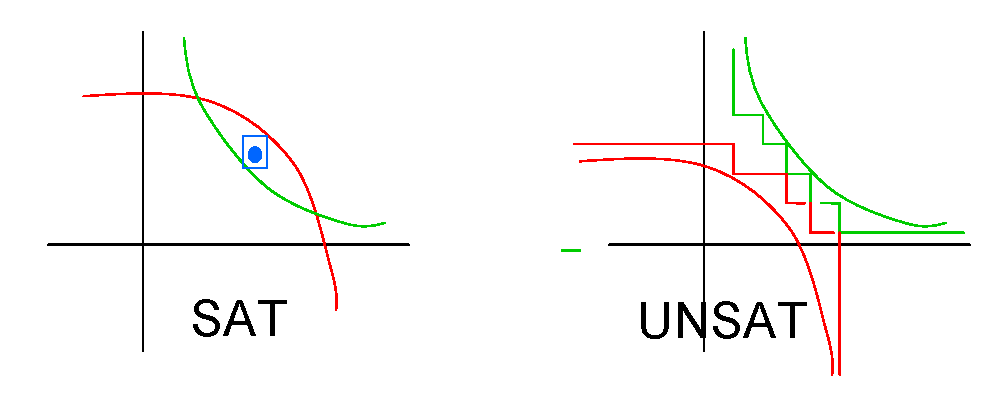
\includegraphics[height=1.2in,width=3.4in]{FigCompleteness.eps} 
\caption{SAT and UNSAT detection by ICP} 
\label{fig:complete} 
%\end{minipage}
\end{figure} 

The boundary part is reduced to polynomial equality checking, 
which would be solved algebraic methods, like Groebner basis. 
Alternatively, by loosening equality to $\delta$-equality, 
$\delta$-completeness is obtained~\cite{dRealIJCAR12,dRealLICS12}. 

This paper presents an SMT solver {\bf raSAT} for polynomial inequality. 
It consists of a simple iterative approximation refinement, called {\bf raSAT} {\em loop}, 
which is an extension of the standard ICP with testing to accelerate SAT detection. 
Two approximation schemes consist of interval arithmetic (over-approximation) and 
testing (under-approximation), to accelerate SAT detection. 
If both fails, input intervals are refined by decomposition. 
%
Compared to typical ICPs, {\bf raSAT} 
\begin{itemize}
\item introduces testing (as an under-approximation) to accelerate SAT detection, 
\item applies various interval arithmetic, e.g., Affine intervals~\cite{Stolfi03,ngocase,tapas12}, 
which enables to analyze the effects of input values, and 
\item SAT confirmation step by an error-bound guaranteed floating point package {\bf iRRAM}\footnote{% 
\tt http://irram.uni-trier.de}, to avoid soundess bugs caused by roundoff errors. 
\end{itemize}
This design is more on SAT detection oriented, since from our preliminary experiences, 
if the target problems have several hundred variables, solvable cases in practice are 
either SAT or UNSAT with small UNSAT core. 
Thus, acceleration of SAT detection and finding UNSAT core will be keys for scalability. 

ICP is robust for larger degrees, but the number of boxes (products of intervals) to explore 
exponentially explodes when variables increase. 
Thus, design of strategies for selecting variables to decompose and boxes to explore is crucial 
for efficiency. Our strategy design is, 
\begin{itemize}
\item a box with more possiblity to be SAT is selected to explore, which is estimated by 
several heuristic measures, called {\em SAT likelyhood}, 
and the number of unsolved atomic polynomial constraints, and
\item a more influential variable is selected for multiple test cases and decomposition, 
which is estimated by {\em sensitivity}. 
\end{itemize} 
Note that {\em SAT likelyhood} and {\em sensitivity} are estimated during interval arithmetic. 
Especially, the latter can be applied only with Affine intervals. 
{\bf raSAT} also applies incremental search, which is often faster in practice. 
\begin{itemize}
\item {\bf Incremental widening}. 
Starting {\bf raSAT} loop with a smaller interval, and if it is UNSAT, enlarge the input intervals
and restart. 
\item {\bf Incremental deepening}. 
Starting with the bound that each interval will be decomposed no smaller than it. 
If neither SAT nor UNSAT is detected, take a smaller bound and restart. 
\end{itemize} 
Efficient UNSAT core and UNSAT confirmation % with error bound guaranteed floating point arithmetic 
are left for future work. 

They are compared on Zankl and Meti-Tarski benchmarks from 
QF\_NRA category of SMT-LIB\footnote{\tt http://www.smtlib.org/}. 
They are also evaluated by comparing 
{\bf Z3 4.3}\footnote{\tt http://z3.codeplex.com} and {\bf iSAT3}. 
Another advantage of {\bf raSAT} is the ease to handle mixed intergers, 
and experiments on AProVE benchmark from QF\_NIA category of SMT-LIB compares {\bf raSAT} with 
{\bf Z3 4.3}. 
Although {\bf Z3 4.3} performs the best, {\bf raSAT} shows comparable SAT detection on 
very large problems (e.g., with several hundred variables) with the combination of 
{\em SAT likelyhood} and {\em sensitivity}. 


\medskip 
{\bf raSAT} applies SAT confirmation to avoid soundness errors caused by roundoff/overflow errors. 
Another static analysis based approach is found in~\cite{SilvaTACAS12}. 
\end{comment}

\section{Thesis outline}
Coming soon...

\chapter{Over-Approximation and Under-Approximation}
\section{Approximation Theory}
\begin{comment}
$F = \exists x_1 \in I_1 \cdots x_n \in I_n. \bigwedge \limits_j \psi_j(x_1,\cdots,x_n)$, 
%\exists x_1 \ldots x_n. (\underbrace{\bigwedge \limits_i x_i \in I_i}_{I}) \wedge 
%                       (\underbrace{\bigwedge \limits_j \psi_j(x_1,\cdots,x_n)}_{P})
where $\psi_j(x_1,\cdots,x_n)$ is an atomic formula. 
%
$F$ is equivalnet to 
$\exists x_1 \ldots x_n. (\bigwedge \limits_i x_i \in I_i) \wedge (\bigwedge \limits_j \psi_j(x_1,\cdots,x_n))$, 
and we call $\bigwedge \limits_i x_i \in I_i$ {\em interval constraints}, and 
we refer $\bigwedge \limits_j \psi_j(x_1,\cdots,x_n)$ by $\psi(x_1,\cdots,x_n)$. 
Initially, interval constraints have a form of the conjunction $\bigwedge \limits_i x_i \in I_i$, 
and later by refinement, $x_i \in I_i$ is decomposed into a clause $\bigvee_j x_i \in I_{i_j}$, 
which makes a CNF. 

As an SMT (SAT modulo theory) problem, 
boolean variables are assigned to each $x_i \in I_{i_j}$, 
and truth assignments is produced by a SAT solver, 
which are proved or disproved by a background theory $T$ whether it satisfies $\psi(x_1,\cdots,x_n)$. 

As notational convention, $m$ (the lower case) denotes 
a variable assignments on $x_i$'s, and 
$M$ (the upper case) denotes a truth assignment on $x_i \in I_{i_j}$'s. 
We write $m \in M$ when an instance $m = \{ x_i \leftarrow c_i \}$ satisfies 
all $c_i \in I_{i_j}$ that are assigned true by $M$. 

We assume {\em very lazy theory learning}~\cite{dpll}, and 
a backend theory $T$ is applied only for a full truth assignment $M$. 
%We regard $M$ as a conjunction $\bigwedge \limits_i x_i \in I_{i_j}$. 
\begin{itemize}
\item If an instance $m$ satisfies $\psi(x_1,\cdots,x_n)$, we denote $m \models_T \psi(x_1,\cdots,x_n)$. 
\item If each instance $m$ with $m \in M$ satisfies $\psi(x_1,\cdots,x_n)$, 
we denote $M \models_T \psi(x_1,\cdots,x_n)$. 
\end{itemize}
\end{comment}

\begin{comment}
\begin{definition} \label{def:app}
Let $F = \exists x_1 \in I_1 \cdots x_n \in I_n. \psi(x_1,\cdots,x_n)$. 
For a truth assignment on $M$, $F$ is 
\begin{itemize}
\item $T$-valid if $M \models_T \psi(x_1,\cdots,$ $x_n)$, 
\item $T$-satisfiable ($T$-SAT) if $m \models_T \psi(x_1,\cdots,x_n)$ 
for some $m \in M$, and 
\item $T$-unsatisfiable ($T$-UNSAT) if $M \models_T \neg \psi(x_1,\cdots,x_n)$. 
\end{itemize}
If $T$ is clear from the context, we simply say valid, satisfiable, and unsatisfiable. 
\end{definition}
\end{comment}

%%%%%%%%%%%%%
\suppress{
Then, Fig. \ref{fig:T_result} illustrates Definition~\ref{def:app}. 
\begin{figure} [ht]
\centering
\begin{minipage}[b]{0.45\linewidth}
  \includegraphics[height=1.8in,width=1.9in]{T_result.eps}
\caption{Results of a target constraint $F$ in a theory $T$}
\label{fig:T_result}
\end{minipage}
\quad
\begin{minipage}[b]{0.45\linewidth}
   \includegraphics[height=2.2in,width=2.3in]{frame_app.eps}
\caption{{\bf raSAT} loop}
\label{fig:frame}
\end{minipage}
\end{figure}
}
%%%%%%%%%%%%%%%%%%%%%%%%%%%%%%%%

\begin{definition} \label{def:ApproxTheory}
Let $T, T'$ be $\Sigma$-theories and $\varphi$ be any $\Sigma$-formula. 
\begin{itemize}
\item $T'$ is an {\em over-approximation theory} (of $T$) 
iff $T'$-UNSAT of $\varphi$ implies $T$-UNSAT of $\varphi$.
\item $T'$ is an {\em under-approximation theory} (of $T$)
iff $T'$-SAT of $\varphi$ implies $T$-SAT of $\varphi$. 
\end{itemize}
\end{definition}

\begin{theorem}
If $T_O$ be an over-approximation theory of $T$, then for any $\Sigma$-formula $\varphi$: $\varphi$ is $T_O$-VALID $\implies \varphi$ is $T$-VALID.
\end{theorem}

\begin{proof}
$\varphi$ is $T_O$-VALID $\implies$ $\neg\varphi$ is $T_O$-UNSAT (Lemma \ref{lemma:theory-valid-unsat}) $\implies \neg\varphi$ is $T$-UNSAT (Definition \ref{def:ApproxTheory}) $\implies \varphi$ is T-VALID (Lemma \ref{lemma:theory-valid-unsat})
\end{proof}

%Note that $O.T$-valid can be regarded as $U.T$, since $O.T$-valid implies $T$-valid, thus $T$-SAT. 
A typical ICP applies $O.T$ only as an interval arithmetic. 
Later in Section~\ref{sec:approximation}, we will instantiate interval arithmetic as $O.T$. 
Adding to $O.T$-valid, {\bf raSAT} introduce testing as $U.T$ to accelerate SAT detection. 

\section{Interval Arithmetic as an Over-Approximation Theory}
A model $M^p_{IA} = (U^p_{IA}, I^p_{IA})$ over intervals contains a set of all intervals $U^p_{IA} = \{[l, h] | l, h \in \mathbb{R} \text{ and } l <= h\}$ and a map $I^p_{IA}$ that satisfies the following conditions.
\begin{enumerate}
\item $I^p_{IA}(Real) = U^p_{IA}$
\item $\forall p \in P^p$; $I^p_{IA}(p)= U^p_{IA} \times U^p_{IA} \mapsto U^p_{IA}$ where $I^p_{IA}(p)(i_1, i_2) = i_1 \; p_{IA} \; i_2$. The definition of $ p_{IA}$ is as follow:
\begin{itemize}
\item $[l_1, h_1] \succ_{IA} [l_2,  h_2] = true \iff l_1 > h_2$
\item $[l_1, h_1] \succ_{IA} [l_2,  h_2] = false \iff h_1 \le l_2$
\item $[l_1, h_1] \prec_{IA} [l_2,  h_2] = true \iff h_1 < l_2$
\item $[l_1, h_1] \prec_{IA} [l_2,  h_2] = false \iff l_1 \ge h_2$
\item $i_1 \succeq_{IA} i_2 = \neg(i_1 \prec_{IA} i_2)$
\item $i_1 \preceq_{IA} i_2 = \neg(i_1 \succ_{IA} i_2)$
\item $i_1 \approx_{IA} i_2 = i_1 \succeq_{IA} i_2 \wedge i_1 \preceq_{IA} i_2$
\item $i_1 \not\approx_{IA} i_2 = \neg(i_1 \approx_{IA} i_2)$
\end{itemize}
\item $\forall f \in F^p \setminus \{\mathbf{1}\}$; $I^p_{IA}(f) = U^p_{IA} \times U^p_{IA} \mapsto U^p_{IA}$ such that $ I^p_{IA}(f)(i_1, i_2)= i_1 \; f_{IA} \; i_2$ where $f_{IA}$ satisfies the following properties:
\begin{itemize}
\item $i_1 \oplus_{IA} i_2 \supseteq \{r_1 + r_2| r_1 \in i_1 \text{ and } r_2 \in i_2\}$.
\item $i_1 \ominus_{IA} i_2 \supseteq \{r_1 - r_2| r_1 \in i_1 \text{ and } r_2 \in i_2\}$.
\item $i_1 \otimes_{IA} i_2 \supseteq \{r_1 * r_2| r_1 \in i_1 \text{ and } r_2 \in i_2\}$.
\end{itemize}
\item $I^p_{IA}(\mathbf{1}) = [1,1]$
\item $\forall v \in V$; $I^p_{IA} \in U^p_{IA}$
\end{enumerate}
Theory $T^p_{IA} = \{M^p_{IA}| M^p_{IA} \text{ is a model over intervals}\}$. Each model differs to another by the mapping from variables to intervals. As a consequence, one assignment from variables to intervals can be used to describe an model. We denote $\Pi^p_{IA}$ as the model represented by $\Pi = \{x \in [l, h] | v \in V\}$. 

\begin{lemma} \label{lemma:IA-R-OP}
$\forall i_1, i_2 \in U^p_{IA}; \forall r_1 \in i_2, r_2 \in i_2; \forall p \in P^p (i_1 \; p_{IA} \; i_2 = false \implies \neg(r_1 \; p_\mathbb{R} \; r_2))$
\end{lemma}

\begin{proof}
Let $i_1 = [l_1, h_1]$ and $i_2 = [l_2, h_2]$ where $l_1 \le h_1$ and $l_2 \le h_2$. We have: 
\begin{itemize}
\item $r_1 \in i_1 \implies l_1 \le r_1 \le h_1$. 
\item $r_2 \in i_2 \implies l_2 \le r_2 \le h_2$. 
\end{itemize}
Suppose  that $i_1 \; p_{IA} \; i_2 = false$, we need to show $\neg(r_1 \; p_\mathbb{R} \; r_2)$ by considering all the possible cases of $p$:
\begin{enumerate}
\item If $p$ is $\succ$, the we have $[l_1, h_1] \succ_{IA} [l_2, h_2] = false \implies h_1 \le l_2 \implies r_1 \le r_2$ (because $r_1 \le h_1$ and $l_2 \le r_2$) $\implies \neg(r_1 > r2) \implies \neg(r_1 \succ_\mathbb{R} r_2)$.
\item If $p$ is $\prec$, the we have $[l_1, h_1] \prec_{IA} [l_2, h_2] = false \implies l_1 \ge h_2 \implies r_1 \ge r_2$ (because $r_1 \ge l_1$ and $r_2 \le h_2$) $\implies \neg(r_1 < r_2) \implies \neg(r_1 \prec_\mathbb{R} r_2)$.
\item If $p$ is $\succeq$, the we have $[l_1, h_1] \succeq_{IA} [l_2, h_2] = false \implies \neg ([l_1, h_1] \prec_{IA} [l_2, h_2]) = false \implies [l_1, h_1] \prec_{IA} [l_2, h_2] = true \implies h_1 < l_2 \implies r_1 < r_2$ (because $r_1 \le h_1$ and $r_2 \ge l_2$) $\implies \neg(r_1 \ge r_2) \implies \neg(r_1 \succeq_\mathbb{R} r_2)$.
\item If $p$ is $\preceq$, the we have $[l_1, h_1] \preceq_{IA} [l_2, h_2] = false \implies \neg ([l_1, h_1] \succ_{IA} [l_2, h_2]) = false \implies [l_1, h_1] \succ_{IA} [l_2, h_2] = true \implies l_1 > h	_2 \implies r_1 > r_2$ (because $r_1 \ge l_1$ and $r_2 \le h_2$) $\implies \neg(r_1 \le r_2) \implies \neg(r_1 \preceq_\mathbb{R} r_2)$.
\item If $p$ is $\approx$, the we have $i_1 \approx_{IA} i_2 = false \implies i_1 \succeq_{IA} i_2 \wedge i_1 \preceq_{IA} i_2 = false \implies i_1 \succeq_{IA} i_2 = false \text{ or } i_1 \preceq_{IA} i_2 = false \implies r_1 < r_2 \text{ or } r_1 > r_2$ (as the third and fourth case of this proof) $\implies \neg(r_1 = r_2) \implies \neg(r_1 \approx_\mathbb{R} r_2)$.
\item If $p$ is $\not\approx$, the we have $i_1 \not\approx_{IA} i_2 = false \implies \neg(i_1 \approx_{IA} i_2) = false \implies \neg(i_1 \succeq_{IA} i_2 \wedge i_1 \preceq_{IA} i_2) = false \implies \neg(i_1 \succeq_{IA} i_2) \vee \neg(i_1 \preceq_{IA} i_2) = false \implies i_1 \prec_{IA} i_2 \vee i_1 \succ_{IA} i_2 = false \implies i_1 \prec_{IA} i_2 = false \text{ and } i_1 \succ_{IA} i_2 = false \implies r_1 \ge r_2 \text{ and } r_1 \le r_2$ (as the first and second case of this proof) $\implies r_1 = r_2 \implies \neg(r_1 \not= r_2) \implies \neg(r_1 \not\approx_\mathbb{R} r_2)$.
\end{enumerate}
\end{proof}

\begin{theorem} \label{theorem:IA-OverAprox}
If $\Pi = \{v \in [l, h] | v \in V\}$ is a map from variables to intervals, then $\{\Pi^p_{IA}\}$ is an over-approximation of $\Pi^p_\mathbb{R}$.
\end{theorem}

\begin{lemma} \label{lemma:IA-OT}
$\forall t \in TERM^p \; \forall M^p_\mathbb{R} \in \Pi^p_\mathbb{R} \; t^{M^p_\mathbb{R}} \in t^{\Pi^p_{IA}}$.
\end{lemma}

\begin{proof}
Proof is done by induction on structure of term.
Let $t \in TERM^p$ and $M^p_\mathbb{R} = (\mathbb{R}, I^p_\mathbb{R}) \in \Pi^p_\mathbb{R}$
\begin{enumerate}
\item If $t = v \in V$, then $t^{M^p_\mathbb{R}} = I^p_\mathbb{R}(v) \in \Pi(v)$ because $M^p_\mathbb{R} \in \Pi^p_\mathbb{R}$. In addition, $t^{\Pi^p_{IA}} = \Pi^p_\mathbb{R}$.
\item If $t = \mathbf{1}$, then $t^{M^p_\mathbb{R}} = 1 \in [1, 1] = t^{\Pi^p_{IA}}$
\item If $t = t_1 \; f \; t_2$ for some $f \in F^p \setminus \{0, 1\}$

$t^{M^p_\mathbb{R}} = t_1^{M^p_\mathbb{R}} \; f_\mathbb{R} \; t_1^{M^p_\mathbb{R}}$

$t^{\Pi^p_{IA}} = t_1^{\Pi^p_{IA}} \; f_{IA} \; t_2^{\Pi^p_{IA}}$

By induction hypothesis, we have $t_1^{M^p_\mathbb{R}} \in t_1^{\Pi^p_{IA}}$ and $t_1^{M^p_\mathbb{R}} \in t_2^{\Pi^p_{IA}}$. In addition, due to the properties of $f_{IA}$: $t_1^{M^p_\mathbb{R}} \; f_\mathbb{R} \; t_1^{M^p_\mathbb{R}} \in t_1^{\Pi^p_{IA}} \; f_{IA} \; t_2^{\Pi^p_{IA}}$, or $t^{M^p_\mathbb{R}} \in t^{\Pi^p_{IA}}$ 
\end{enumerate}
\end{proof}

\begin{proof}
In order to prove Theorem ~\ref{theorem:IA-OverAprox}, we need to prove that $\forall \varphi^p (\varphi^p$ is $\{\Pi^p_{IA}\}$-UNSAT $\implies \varphi^p$ is $\Pi^p_\mathbb{R}$-UNSAT). 

Given an $\Sigma^p$-formula $\varphi^p$ and suppose that $\varphi^p$ is $\{\Pi^p_{IA}\}$-UNSAT.
Suppose $\varphi^p$ is not $\Pi^p_\mathbb{R}$-UNSAT, that means it is either  $\Pi^p_\mathbb{R}$-SAT or  $\Pi^p_\mathbb{R}$-VALID. In either case, there exist at least a model $M^p_\mathbb{R} \in \Pi^p_\mathbb{R}$ such that $\models_{M^p_\mathbb{R}} \varphi^p \iff (\varphi^p)^{M^p_\mathbb{R}}= true$.
\begin{enumerate}
\item If $\varphi^p = p(t_1, t_2)$ for some $p \in P^p$, then $(\varphi^p)^{M^p_\mathbb{R}}= true \implies t_1^{M^p_\mathbb{R}} \; p_\mathbb{R} \; t_2^{M^p_\mathbb{R}}$. 

On the other hand, $\varphi^p$ is $\{\Pi^p_{IA}\}$-UNSAT $\implies (\varphi^p)^{\Pi^p_{IA}} = false \implies t_1^{\Pi^p_{IA}} \; p_{IA} \; t_2^{\Pi^p_{IA}} = false$. In addition, because $t_1^{M^p_\mathbb{R}} \in t_1^{\Pi^p_{IA}}$ and $t_2^{M^p_\mathbb{R}} \in t_2^{\Pi^p_{IA}}$ (Lemma ~\ref{lemma:IA-OT}), $t_1^{\Pi^p_{IA}} \; p_{IA} \; t_2^{\Pi^p_{IA}} = false \implies \neg(t_1^{M^p_\mathbb{R}} \; p_\mathbb{R} \; t_2^{M^p_\mathbb{R}})$ (Lemma ~\ref{lemma:IA-R-OP}). This is a contradiction. As the result, $\varphi^p$ must be $\Pi^p_\mathbb{R}$-UNSAT.
\item If $\varphi^p = \varphi^p_1 \wedge \varphi^p_2$ is  
\end{enumerate}
\end{proof}

\section{Testing as an Under-Approximation Theory}


\section{raSAT loop}
\begin{grammar}
<bound\_atom> ::= <variable> $\in$ [real, real] | <variable> $\in$ (-inf, real] | <variable> $\in$ [real, inf) | <variable> $\in$ (-inf, inf)


<bound\_constraint> ::= $\bigwedge\limits_i\bigvee\limits_jbound\_atom_{ij}$
\end{grammar}
In other word, each model can be represented by an assignment of one real number to each variable. 
State of search procedure contains  $(\Pi, \varphi, \Pi^c, \varphi^V, \varphi^U)$ where 
\begin{itemize}
\item $\Pi$ is the interval constraint
\item $\varphi$ represents the polynomial constraint.
\item $\varphi^V$ contains the constraints that are valid under over-approximation.
\item $\varphi^U$ is the set of constraints which are UNKNOWN under over-approximation.
\end{itemize}
The transition rules are described in Table ~\ref{tab:transition-rules}. Figure ~\ref{fig:smt-design} illustrates the transition system. 

\begin{table*}[t]
  \centering
  \begin{tabular}{ll}
  \hline\\
  \large 
  $\frac{\Pi \models_{SAT} \bot}{(\Pi, \Psi, \emptyset, \emptyset, \emptyset) \to UNSAT}$ \tiny $\Pi$\_UNSAT \\\\
  \large 
  $\frac{\Pi \models_{SAT} \Pi^c \quad \Pi^{c'} = flattern(\Pi^c)}{(\Pi, \Psi, \emptyset, \emptyset, \emptyset) \to (\Pi, \Psi, \Pi^{c'}, \emptyset, \emptyset)}$ \tiny $\Pi$\_SAT\\\\
  $\frac{\Pi^c \not= \emptyset \quad \Psi^V \subseteq \Psi \quad \Psi^U \subseteq \Psi \quad \Psi^V \cap \Psi^U = \Psi \quad \Psi^V \cup \Psi^U = \emptyset \quad \Psi^V \text{ is }  T_O\text{-VALID} \quad \Psi^U \text{ is }  T_O\text{-SAT}}{(\Pi, \Psi, \Pi^c, \emptyset, \emptyset) \to (\Pi, \Psi, \Pi^c, \Psi^V, \Psi^U)}$ \tiny $T_O$\_SAT \\\\  
  \large 
  $\frac{\Psi^V = \Psi}{(\Pi, \Psi, \Pi^c, \Psi^V, \Psi^U) \to SAT}$ \tiny $T_O$\_VALID \\\\
  \large 
  $\frac{\Pi^c \not= \emptyset \quad \Psi^U \not= \emptyset \quad \Psi^U \text{ is }  T^U\text{-SAT}}{(\Pi, \Psi, \Pi^c, \Psi^V, \Psi^U) \to SAT}$ \tiny $T^U$\_SAT \\\\
  \large 
  $\frac{\Psi^U \text{ is }  T^U\text{-UNSAT} \quad \varphi \in \Psi^U \quad x_j \in \varphi \quad (I_j = x_j \in [l_j, h_j]) \in \Pi^c \quad l_j < d \in \mathbb{R} < h_j \quad I_{j1} = x_j \in [l_j, d] \quad I_{j2} = x_j \in [d, h_j]}{(\Pi, \Psi, \Pi^c, \Psi^V, \Psi^U) \to (\Pi \wedge (\neg I_j \vee I_{j1} \vee I_{j2}) \wedge (I_j \vee \neg I_{j1}) \wedge (I_j \vee \neg I_{j2}) \wedge (\neg I_{j1} \vee \neg I_{j2}), \Psi, \emptyset, \emptyset, \emptyset)}$ \tiny REFINE \\\\
  \large 
  $\frac{\{\varphi_i| i = 1,\cdots, n; \; \varphi_i \text{ is } T_O\text{-UNSAT}\} \subseteq \Psi \quad var(\varphi_i) = \{x_{ij}|j=1,\cdots, m_i\} \quad (I_{ij} = x_{ij} \in [l_{ij}, h_{ij}]) \in \Pi^c}{(\Pi, \Psi, \Pi^c, \emptyset, \emptyset) \to (\Pi \wedge \bigwedge\limits_{i=1}^n \bigvee\limits_{j=1}^{m_i} \neg I_{ij}, \Psi, \emptyset, \emptyset, \emptyset)}$ \tiny $T_O$\_UNSAT \\\\
  \hline\\
  \end{tabular}
  \caption{Transition rules}\label{tab:transition-rules}
\end{table*}

\section{Soundness - Completeness}
\begin{comment}
\section{Over-Approximation Theory Refinement}
\label{sec:soundness}

From now on, We focus on a \emph{polynomial inequality} such that 
$I_i$ and $\psi_j(x_1,\cdots,x_n)$ are an open interval $(a_i,b_i)$ and 
an atomic polynomial inequaltiy (API) $f_j > 0$, respectively. 
We denote $\mathbb{S}(f_j) = \{x \in \Real^n \mid f_j > 0 ~\text{holds}\}$.

For ICP, it is folklore that, for polynomial inequality 
$\exists x_1 \in (a_1,b_1) \cdots x_n \in (a_n,b_n) . \wedge_{i} f_i > 0$, 
\begin{itemize}
\item if $\exists x_1 \in (a_1,b_1) \cdots x_n \in (a_n,b_n) . \wedge_{i} f_i > 0$ is SAT, 
ICP eventually detects it, and 
\item if $\exists x_1 \in [a_1,b_1] \cdots x_n \in [a_n,b_n] . \wedge_{i} f_i \geq 0$ is UNSAT, 
ICP eventually detects it, 
\end{itemize}
under the assumptions of {\em fair} decomposition and bounded intervals $(a_i,b_i)$. 
We will prepare terminology and briefly review this fact. 

%%%%%%%%%%%%%%%%%%%%%%
\suppress{
\begin{definition} \label{def:poly}
A polynomial inequality is a bounded quantification 
$\exists x_1 \in I_1 \cdots x_n \in I_n. \psi(x_1,\cdots,x_n)$ 
such that 
\begin{itemize}
\item each $I_i$ is an open interval $x_i \in (a_i,b_i)$, and 
\item $\psi(x_1,\cdots,x_n)$ is a conjunction of $f_j > 0$ 
where $f_j$ is a polynomial over $\{x_1, \cdots, x_n\}$. 
\end{itemize}
$f_i > 0$ is called an atomic polynomial inequality (API). 
We denote $\mathbb{S}(F) = \{x \in \Real^n \mid F ~\text{holds}\}$.
\end{definition}

\begin{example} \label{examp:poly_ieq}
$\exists x \in (-1,3)~y \in (2,4) . (x^3y - y^4 > 0) \wedge (y^3 -xy >0)$
is an example of a polynomial inequality with 2 variables and 2 APIs. 
\end{example}
}
%%%%%%%%%%%%%%%%%%%%%%

\begin{definition}
An \emph{open box} of dimension $n$ is a set $(a_1,b_1) \times \cdots \times (a_n,b_n)$ 
where $a_i, b_i \in \Real, a_i \leq b_i$.  
For $\mathfrak{a} = (a_1, \cdots, a_n)$ and $\mathfrak{b} = (b_1, \cdots, b_n)$, 
we denote $(a_1,b_1) \times \cdots \times (a_n,b_n)$ by $(\mathfrak{a}, \mathfrak{b})$. 
\end{definition}

The set of all open boxes is a basis of Euclidean topology on $\Real^n$. 
In $\Real^n$, a set $U$ is compact if, and only if, $U$ is a bounded closed set. 
We denote a closure of a set $U$ by $\overline{U}$. 
%
Since a polynomial is continuous, 
$\mathbb{S}(\bigwedge \limits_{i=1}^m f_i > 0)$ is an open set. 
Note that $\Rat$ is dense in $\Real$, and an SAT instance in reals can be replaced with one in rationals. 

%%%%%%%%%%%%%%%%%%%%%%%%%%%%%%
\suppress{
\begin{lemma} \label{cor:rattoreal}
For a polynomial inequality
$F = \exists x_1 \in I_1 \cdots x_n \in I_n. \bigwedge \limits_{j=1}^m f_j > 0$, 
If there exists an SAT instance of F in $\Real^n$, there exists also in $\Rat^n$. 
\end{lemma}

\begin{lemma} \label{cor:refinement}
Suppose that $a_j < b_j$ for $1 \leq j \leq n$ and $f_i$'s are polynomials. 
Assume $a_k < c < b_k$ for some $k$. 
Then, 
$\exists x_1 \in (a_1,b_1) \cdots x_n \in (a_n,b_n). \bigwedge \limits_{i=1}^m f_i > 0$ 
is SAT (resp. UNSAT) if, and only if, 
$\exists x_1 \in (a_1,b_1) \cdots x_k \in (a_k,c) \cdots x_n \in (a_n,b_n). 
 \bigwedge \limits_{i=1}^m f_i > 0 
 \vee 
 \exists x_1 \in (a_1,b_1) \cdots x_k \in (c,b_k) \cdots x_n \in (a_n,b_n)). 
 \bigwedge \limits_{i=1}^m f_i > 0$ 
is SAT (resp. UNSAT). 
\end{lemma}

\begin{pf}
We show for the SAT case. If-part is obvious. For only-if-part, 
since $\mathbb{S}(\bigwedge \limits_{i=1}^m f_i > 0)$ is an open set, 
if $y \in (a_1,b_1) \times \cdots \{c\} \cdots \times (a_n,b_n)$ satisfies 
$\bigwedge \limits_{i=1}^m f_i > 0$, 
there exists $x_1 \in (a_1,b_1) \cdots x_k \in (a_k,c) \cdots x_n \in (a_n,b_n)$
(also $x_1 \in (a_1,b_1) \cdots x_k \in (c,b_k) \cdots x_n \in (a_n,b_n)$) that satisfies
$\bigwedge \limits_{i=1}^m f_i > 0$. 
\end{pf}

Lemma~\ref{cor:rattoreal} says that proving SAT of $F$ in $\Real$ is reduced to 
that in $\Rat$. 
Lemma~\ref{cor:refinement} says that, in the refinement step, we can apply refinement 
$x_k \in (a_k,b_k)$ to $x_k \in (a_k,c) \vee x_k \in (c,b_k)$, 
instead of $x_k \in (a_k,c] \vee x_k \in (c,b_k) $
(i.e., $c$ is ignored). 
}
%%%%%%%%%%%%%%%%%%%%%%%%%%%%%%

Initially, interval constraints consists of conjunction only. Later, by refinements, it becomes a CNF. 


%\begin{example} \label{examp:poly_ieq}
$\exists x \in (-1,3)~y \in (2,4) . (x^3y - y^4 > 0) \wedge (y^3 -xy >0)$
is an example of a polynomial inequality with 2 variables and 2 APIs. 

For instance, $x \in (-1,3)$ and $y \in (2,4)$ are refined to smaller intervals
such that 
$\exists x \in (-1,1) y \in (2,4) . (x^3y - y^4 > 0) \wedge (y^3 -xy >0) \vee 
 \exists x \in (1,3) y \in (2,4) . (x^3y - y^4 > 0) \wedge (y^3 -xy >0)$, 
which results a CNF 
$(x \in (-1,1) \vee x \in (1,3)) \wedge (y \in (2,4)) \wedge (x^3y - y^4 > 0) \wedge (y^3 -xy >0)$.
%(only the CNF formula $(x \in (-1,1) \vee x \in (1,3)) \wedge (y \in (2,4))$ is given to SAT solver).
%\mizuhito{could you fulfill? Direct encoding seems a DNF?}. 
%\end{example}

Note that an interval arithmetic used in ICP is a converging theory. 

\begin{definition} \label{def:completeOT}
Let
$F = \exists x_1 \in I_1 \cdots x_n \in I_n. \bigwedge \limits_{j=1}^m f_j > 0$
be a polynomial inequality such that each $I_i$ is bounded. 
An over-approximation theory $O.T$ is {\em converging} 
if, for each $\delta > 0$ and $c = (c_1, \cdots, c_n) \in I_1 \times \cdots \times I_n$, 
there exists $\gamma > 0$ such that 
$\bigwedge \limits_{j=1}^n x_j \in (c_j - \gamma, c_j + \gamma) \models_{O.T} 
 \bigwedge \limits_{i=1}^m (f_i(c) - \delta < f_i(x) < f_i(c) + \delta)$. 
\end{definition}

$O.T$ refinemnet loop is shown in Fig.~\ref{fig:OTrefine}~(a). 
A standard ICP based algorithm of an SMT solver applies it with $O.T$ as a classical interval arithemtic. 
The variation of interval arithemtic will be presented in Section~\ref{sec:approximation}. 
\begin{figure}[ht]
\begin{minipage}[b]{1.0\linewidth}
\centering
\begin{tabular}{c@{\quad}c}
\includegraphics[height=0.6in,width=1.7in]{OTloop.png} & 
\includegraphics[height=0.9in,width=1.7in]{rasatloop.png} \\   
\mbox{(a) $O.T$ refinement loop} & \mbox{{\bf raSAT} loop} \\
\end{tabular}
\end{minipage} 
\caption{Rfinement loops} 
\label{fig:OTrefine} 
\end{figure}


\begin{definition} 
Let
$F = \exists x_1 \in I_1 \cdots x_n \in I_n. \bigwedge \limits_{j=1}^m f_j > 0$
for $I_i = (a_i,b_i)$.
A refinement strategy is {\em fair}, if, for each $c_j \in (a_j,b_j)$ and $\gamma > 0$, 
a decomposition of $I_i$ for each $i$ eventually occurs in $(c_j - \gamma, c_j + \gamma)$ 
(as long as neither SAT nor UNSAT is detected). 
\end{definition}

\begin{theorem} \label{th:RelComp}
Let
$F = \exists x_1 \in I_1 \cdots x_n \in I_n. \bigwedge \limits_{j=1}^m f_j > 0$
for $I_i = (a_i,b_i)$.
Assume that an over-approximation theory $O.T$ is converging, 
each $(a_i,b_i)$ is bounded, and a refinement strategy is fair. 
Then, 
\begin{itemize}
\item if $\exists x_1 \in (a_1,b_1) \cdots x_n \in (a_n,b_n) . \wedge_{i} f_i > 0$ is SAT, 
$O.T$ refinemnet loop eventually detects it, and
\item if $\exists x_1 \in [a_1,b_1] \cdots x_n \in [a_n,b_n] . \wedge_{i} f_i \geq 0$ is UNSAT, 
$O.T$ refinement loop eventually detects it.  
\end{itemize}
\end{theorem}


\begin{proof} 
The former is proved by the fact that, if $F$ is SAT, there exists a non-empty neiborhood (open box) 
in $\cap~\mathbb{S}(f_j)$. 
If the box decomposition strategy is fair, the refinemnet will eventually find such an open box. 

For the latter, assume that 
$\overline{F} = \exists x_1 \in [a_1,b_1] \cdots x_n \in [a_n,b_n] . \wedge_{i} f_i \geq 0$ is UNSAT. 
Thus, $\cap~\overline{\mathbb{S}(f_i)} = \emptyset$. 
Let $\delta_{j,k} = min \{|f_j(\bar{x}) - f_k(\bar{x})| \mid \bar{x} \in I_1 \times \cdots \times I_n\}$. 
Since $f_i$'s are continuous and $\overline{I_i}$'s are compact, $\delta_{j,k}$ is well defined,
and $\delta_{j.k} > 0$ for some $j,k$. 
Let $\delta = \frac{min \{ \delta_{j,k} \}}{2}$. 
Since $O.T$ is converging, there exists $\gamma > 0$ for $\delta > 0$ 
satisfying Definition~\ref{def:completeOT}, and fair decomposition eventually finds open boxes
such that $\mathbb{S}(f_j)$ and $\mathbb{S}(f_k)$ are separated. 
%\qed
\end{proof}

Limitations for detecting UNSAT occur on \emph{kissing} and \emph{convergent} cases. 
Fig.~\ref{fig:limit} left shows a kissing case 
$x^2 + y^2 < 2^2 \wedge (x-4)^2 + (y-3)^2 < 3^2$ such that 
$\overline{\mathbb{S}(- x^2 - y^2 + 2^2)} \cap \overline{\mathbb{S}(- (x-4)^2 - (y-3)^2 + 3^2)} 
= \{(x,y) \mid (1.6, 1.2)\}$. 
Thus, there are no coverings to separate them. 
%$x^2 + y^2 < 2^2$ and $(x-4)^2 + (y-3)^2 < 3^2$. 
%
Fig. \ref{fig:limit} right shows a convergent case 
$y > x + \frac{1}{x} \wedge y < x \wedge x > 0$, which is equivalent to 
$xy > x^2 + x \wedge y < x \wedge x > 0$. 
%The open box is $(0,\infty) \times (0,\infty)$ and 
There are no finite coverings to separate them. 
%$y > x + \frac{1}{x}$ and $y < x$ for $x > 0$. 

\begin{figure}[ht]
%\begin{minipage}[b]{1.0\linewidth}
\centering
\begin{tabular}{cc}
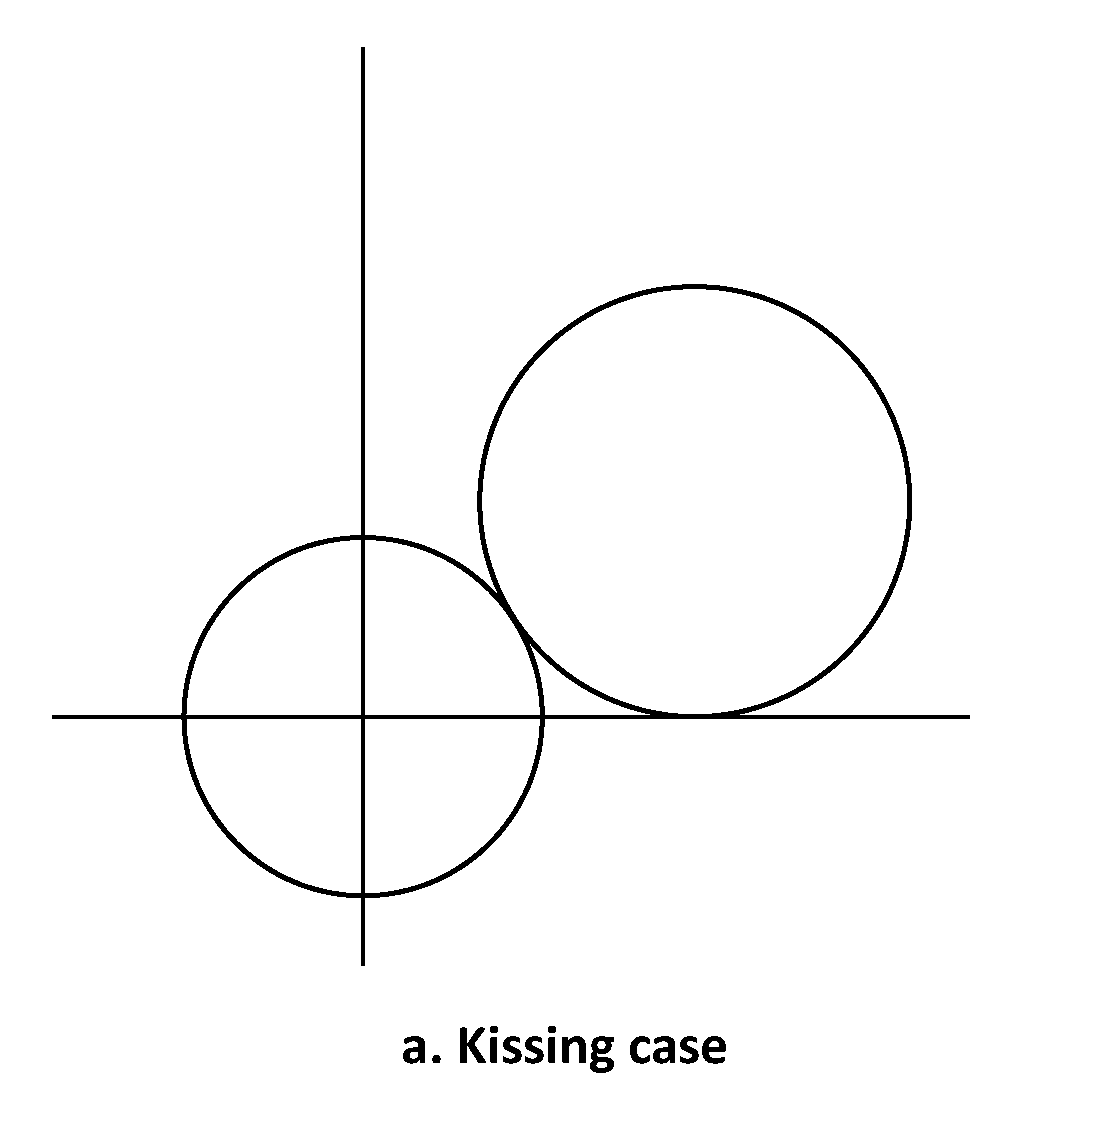
\includegraphics[height=1.65in,width=1.7in]{kissing.eps} &
\includegraphics[height=1.65in,width=1.7in]{convergence.eps}
\end{tabular}
\caption{Limitations for proving UNSAT} 
\label{fig:limit} 
%\end{minipage}
\end{figure} 
\end{comment}

\chapter{Soundness - Completeness}
Coming soon...
\section{Soundness}
Coming soon...
\section{Completeness}
Coming soon...

\chapter{Over and Under-approximation for polynomials}
Let 
$F = \exists x_1 \in I_1 \cdots x_n \in I_n. \bigwedge \limits_j \psi_j(x_1,\cdots,x_n)$, 
%\exists x_1 \ldots x_n. (\underbrace{\bigwedge \limits_i x_i \in I_i}_{I}) \wedge 
%                       (\underbrace{\bigwedge \limits_j \psi_j(x_1,\cdots,x_n)}_{P})
where $\psi_j(x_1,\cdots,x_n)$ is an atomic formula. 
%
$F$ is equivalnet to 
$\exists x_1 \ldots x_n. (\bigwedge \limits_i x_i \in I_i) \wedge (\bigwedge \limits_j \psi_j(x_1,\cdots,x_n))$, 
and we call $\bigwedge \limits_i x_i \in I_i$ {\em interval constraints}, and 
we refer $\bigwedge \limits_j \psi_j(x_1,\cdots,x_n)$ by $\psi(x_1,\cdots,x_n)$. 
Initially, interval constraints have a form of the conjunction $\bigwedge \limits_i x_i \in I_i$, 
and later by refinement, $x_i \in I_i$ is decomposed into a clause $\bigvee_j x_i \in I_{i_j}$, 
which makes a CNF. 

As an SMT (SAT modulo theory) problem, 
boolean variables are assigned to each $x_i \in I_{i_j}$, 
and truth assignments is produced by a SAT solver, 
which are proved or disproved by a background theory $T$ whether it satisfies $\psi(x_1,\cdots,x_n)$. 

As notational convention, $m$ (the lower case) denotes 
a variable assignments on $x_i$'s, and 
$M$ (the upper case) denotes a truth assignment on $x_i \in I_{i_j}$'s. 
We write $m \in M$ when an instance $m = \{ x_i \leftarrow c_i \}$ satisfies 
all $c_i \in I_{i_j}$ that are assigned true by $M$. 

We assume {\em very lazy theory learning}~\cite{dpll}, and 
a backend theory $T$ is applied only for a full truth assignment $M$. 
%We regard $M$ as a conjunction $\bigwedge \limits_i x_i \in I_{i_j}$. 
\begin{itemize}
\item If an instance $m$ satisfies $\psi(x_1,\cdots,x_n)$, we denote $m \models_T \psi(x_1,\cdots,x_n)$. 
\item If each instance $m$ with $m \in M$ satisfies $\psi(x_1,\cdots,x_n)$, 
we denote $M \models_T \psi(x_1,\cdots,x_n)$. 
\end{itemize}

\begin{definition} \label{def:app}
Let $F = \exists x_1 \in I_1 \cdots x_n \in I_n. \psi(x_1,\cdots,x_n)$. 
For a truth assignment on $M$, $F$ is 
\begin{itemize}
\item $T$-valid if $M \models_T \psi(x_1,\cdots,$ $x_n)$, 
\item $T$-satisfiable ($T$-SAT) if $m \models_T \psi(x_1,\cdots,x_n)$ 
for some $m \in M$, and 
\item $T$-unsatisfiable ($T$-UNSAT) if $M \models_T \neg \psi(x_1,\cdots,x_n)$. 
\end{itemize}
If $T$ is clear from the context, we simply say valid, satisfiable, and unsatisfiable. 
\end{definition}

%%%%%%%%%%%%%
\suppress{
Then, Fig. \ref{fig:T_result} illustrates Definition~\ref{def:app}. 
\begin{figure} [ht]
\centering
\begin{minipage}[b]{0.45\linewidth}
  \includegraphics[height=1.8in,width=1.9in]{T_result.eps}
\caption{Results of a target constraint $F$ in a theory $T$}
\label{fig:T_result}
\end{minipage}
\quad
\begin{minipage}[b]{0.45\linewidth}
   \includegraphics[height=2.2in,width=2.3in]{frame_app.eps}
\caption{{\bf raSAT} loop}
\label{fig:frame}
\end{minipage}
\end{figure}
}
%%%%%%%%%%%%%%%%%%%%%%%%%%%%%%%%

\begin{definition} \label{def:ApproxTheory}
Let $T, O.T, U.T$ be theories. 
\begin{itemize}
\item $O.T$ is an {\em over-approximation theory} (of $T$) 
if $O.T$-UNSAT implies $T$-UNSAT, and
\item $U.T$ is an {\em under-approximation theory} (of $T$)
if $U.T$-SAT implies $T$-SAT. 
\end{itemize}
We further assume that $O.T$-valid implies $T$-valid. 
\end{definition}

%Note that $O.T$-valid can be regarded as $U.T$, since $O.T$-valid implies $T$-valid, thus $T$-SAT. 
A typical ICP applies $O.T$ only as an interval arithmetic. 
Later in Section~\ref{sec:approximation}, we will instantiate interval arithmetic as $O.T$. 
Adding to $O.T$-valid, {\bf raSAT} introduce testing as $U.T$ to accelerate SAT detection. 



\subsection{Over-Approximation Theory Refinement}
\label{sec:soundness}

From now on, We focus on a \emph{polynomial inequality} such that 
$I_i$ and $\psi_j(x_1,\cdots,x_n)$ are an open interval $(a_i,b_i)$ and 
an atomic polynomial inequaltiy (API) $f_j > 0$, respectively. 
We denote $\mathbb{S}(f_j) = \{x \in \Real^n \mid f_j > 0 ~\text{holds}\}$.

For ICP, it is folklore that, for polynomial inequality 
$\exists x_1 \in (a_1,b_1) \cdots x_n \in (a_n,b_n) . \wedge_{i} f_i > 0$, 
\begin{itemize}
\item if $\exists x_1 \in (a_1,b_1) \cdots x_n \in (a_n,b_n) . \wedge_{i} f_i > 0$ is SAT, 
ICP eventually detects it, and 
\item if $\exists x_1 \in [a_1,b_1] \cdots x_n \in [a_n,b_n] . \wedge_{i} f_i \geq 0$ is UNSAT, 
ICP eventually detects it, 
\end{itemize}
under the assumptions of {\em fair} decomposition and bounded intervals $(a_i,b_i)$. 
We will prepare terminology and briefly review this fact. 

%%%%%%%%%%%%%%%%%%%%%%
\suppress{
\begin{definition} \label{def:poly}
A polynomial inequality is a bounded quantification 
$\exists x_1 \in I_1 \cdots x_n \in I_n. \psi(x_1,\cdots,x_n)$ 
such that 
\begin{itemize}
\item each $I_i$ is an open interval $x_i \in (a_i,b_i)$, and 
\item $\psi(x_1,\cdots,x_n)$ is a conjunction of $f_j > 0$ 
where $f_j$ is a polynomial over $\{x_1, \cdots, x_n\}$. 
\end{itemize}
$f_i > 0$ is called an atomic polynomial inequality (API). 
We denote $\mathbb{S}(F) = \{x \in \Real^n \mid F ~\text{holds}\}$.
\end{definition}

\begin{example} \label{examp:poly_ieq}
$\exists x \in (-1,3)~y \in (2,4) . (x^3y - y^4 > 0) \wedge (y^3 -xy >0)$
is an example of a polynomial inequality with 2 variables and 2 APIs. 
\end{example}
}
%%%%%%%%%%%%%%%%%%%%%%

\begin{definition}
An \emph{open box} of dimension $n$ is a set $(a_1,b_1) \times \cdots \times (a_n,b_n)$ 
where $a_i, b_i \in \Real, a_i \leq b_i$.  
For $\mathfrak{a} = (a_1, \cdots, a_n)$ and $\mathfrak{b} = (b_1, \cdots, b_n)$, 
we denote $(a_1,b_1) \times \cdots \times (a_n,b_n)$ by $(\mathfrak{a}, \mathfrak{b})$. 
\end{definition}

The set of all open boxes is a basis of Euclidean topology on $\Real^n$. 
In $\Real^n$, a set $U$ is compact if, and only if, $U$ is a bounded closed set. 
We denote a closure of a set $U$ by $\overline{U}$. 
%
Since a polynomial is continuous, 
$\mathbb{S}(\bigwedge \limits_{i=1}^m f_i > 0)$ is an open set. 
Note that $\Rat$ is dense in $\Real$, and an SAT instance in reals can be replaced with one in rationals. 

%%%%%%%%%%%%%%%%%%%%%%%%%%%%%%
\suppress{
\begin{lemma} \label{cor:rattoreal}
For a polynomial inequality
$F = \exists x_1 \in I_1 \cdots x_n \in I_n. \bigwedge \limits_{j=1}^m f_j > 0$, 
If there exists an SAT instance of F in $\Real^n$, there exists also in $\Rat^n$. 
\end{lemma}

\begin{lemma} \label{cor:refinement}
Suppose that $a_j < b_j$ for $1 \leq j \leq n$ and $f_i$'s are polynomials. 
Assume $a_k < c < b_k$ for some $k$. 
Then, 
$\exists x_1 \in (a_1,b_1) \cdots x_n \in (a_n,b_n). \bigwedge \limits_{i=1}^m f_i > 0$ 
is SAT (resp. UNSAT) if, and only if, 
$\exists x_1 \in (a_1,b_1) \cdots x_k \in (a_k,c) \cdots x_n \in (a_n,b_n). 
 \bigwedge \limits_{i=1}^m f_i > 0 
 \vee 
 \exists x_1 \in (a_1,b_1) \cdots x_k \in (c,b_k) \cdots x_n \in (a_n,b_n)). 
 \bigwedge \limits_{i=1}^m f_i > 0$ 
is SAT (resp. UNSAT). 
\end{lemma}

\begin{pf}
We show for the SAT case. If-part is obvious. For only-if-part, 
since $\mathbb{S}(\bigwedge \limits_{i=1}^m f_i > 0)$ is an open set, 
if $y \in (a_1,b_1) \times \cdots \{c\} \cdots \times (a_n,b_n)$ satisfies 
$\bigwedge \limits_{i=1}^m f_i > 0$, 
there exists $x_1 \in (a_1,b_1) \cdots x_k \in (a_k,c) \cdots x_n \in (a_n,b_n)$
(also $x_1 \in (a_1,b_1) \cdots x_k \in (c,b_k) \cdots x_n \in (a_n,b_n)$) that satisfies
$\bigwedge \limits_{i=1}^m f_i > 0$. 
\end{pf}

Lemma~\ref{cor:rattoreal} says that proving SAT of $F$ in $\Real$ is reduced to 
that in $\Rat$. 
Lemma~\ref{cor:refinement} says that, in the refinement step, we can apply refinement 
$x_k \in (a_k,b_k)$ to $x_k \in (a_k,c) \vee x_k \in (c,b_k)$, 
instead of $x_k \in (a_k,c] \vee x_k \in (c,b_k) $
(i.e., $c$ is ignored). 
}
%%%%%%%%%%%%%%%%%%%%%%%%%%%%%%

Initially, interval constraints consists of conjunction only. Later, by refinements, it becomes a CNF. 


%\begin{example} \label{examp:poly_ieq}
$\exists x \in (-1,3)~y \in (2,4) . (x^3y - y^4 > 0) \wedge (y^3 -xy >0)$
is an example of a polynomial inequality with 2 variables and 2 APIs. 

For instance, $x \in (-1,3)$ and $y \in (2,4)$ are refined to smaller intervals
such that 
$\exists x \in (-1,1) y \in (2,4) . (x^3y - y^4 > 0) \wedge (y^3 -xy >0) \vee 
 \exists x \in (1,3) y \in (2,4) . (x^3y - y^4 > 0) \wedge (y^3 -xy >0)$, 
which results a CNF 
$(x \in (-1,1) \vee x \in (1,3)) \wedge (y \in (2,4)) \wedge (x^3y - y^4 > 0) \wedge (y^3 -xy >0)$.
%(only the CNF formula $(x \in (-1,1) \vee x \in (1,3)) \wedge (y \in (2,4))$ is given to SAT solver).
%\mizuhito{could you fulfill? Direct encoding seems a DNF?}. 
%\end{example}

Note that an interval arithmetic used in ICP is a converging theory. 

\begin{definition} \label{def:completeOT}
Let
$F = \exists x_1 \in I_1 \cdots x_n \in I_n. \bigwedge \limits_{j=1}^m f_j > 0$
be a polynomial inequality such that each $I_i$ is bounded. 
An over-approximation theory $O.T$ is {\em converging} 
if, for each $\delta > 0$ and $c = (c_1, \cdots, c_n) \in I_1 \times \cdots \times I_n$, 
there exists $\gamma > 0$ such that 
$\bigwedge \limits_{j=1}^n x_j \in (c_j - \gamma, c_j + \gamma) \models_{O.T} 
 \bigwedge \limits_{i=1}^m (f_i(c) - \delta < f_i(x) < f_i(c) + \delta)$. 
\end{definition}

$O.T$ refinemnet loop is shown in Fig.~\ref{fig:OTrefine}~(a). 
A standard ICP based algorithm of an SMT solver applies it with $O.T$ as a classical interval arithemtic. 
The variation of interval arithemtic will be presented in Section~\ref{sec:approximation}. 
\begin{figure}[ht]
\begin{minipage}[b]{1.0\linewidth}
\centering
\begin{tabular}{c@{\qquad}c}
\includegraphics[height=0.6in,width=1.7in]{OTloop.png} & 
\includegraphics[height=0.9in,width=1.7in]{rasatloop.png} \\   
\mbox{(a) $O.T$ refinement loop} & \mbox{{\bf raSAT} loop} \\
\end{tabular}
\end{minipage} 
\caption{Rfinement loops} 
\label{fig:OTrefine} 
\end{figure}


\begin{definition} 
Let
$F = \exists x_1 \in I_1 \cdots x_n \in I_n. \bigwedge \limits_{j=1}^m f_j > 0$
for $I_i = (a_i,b_i)$.
A refinement strategy is {\em fair}, if, for each $c_j \in (a_j,b_j)$ and $\gamma > 0$, 
a decomposition of $I_i$ for each $i$ eventually occurs in $(c_j - \gamma, c_j + \gamma)$ 
(as long as neither SAT nor UNSAT is detected). 
\end{definition}

\begin{theorem} \label{th:RelComp}
Let
$F = \exists x_1 \in I_1 \cdots x_n \in I_n. \bigwedge \limits_{j=1}^m f_j > 0$
for $I_i = (a_i,b_i)$.
Assume that an over-approximation theory $O.T$ is converging, 
each $(a_i,b_i)$ is bounded, and a refinement strategy is fair. 
Then, 
\begin{itemize}
\item if $\exists x_1 \in (a_1,b_1) \cdots x_n \in (a_n,b_n) . \wedge_{i} f_i > 0$ is SAT, 
$O.T$ refinemnet loop eventually detects it, and
\item if $\exists x_1 \in [a_1,b_1] \cdots x_n \in [a_n,b_n] . \wedge_{i} f_i \geq 0$ is UNSAT, 
$O.T$ refinement loop eventually detects it.  
\end{itemize}
\end{theorem}


\begin{proof} 
The former is proved by the fact that, if $F$ is SAT, there exists a non-empty neiborhood (open box) 
in $\cap~\mathbb{S}(f_j)$. 
If the box decomposition strategy is fair, the refinemnet will eventually find such an open box. 

For the latter, assume that 
$\overline{F} = \exists x_1 \in [a_1,b_1] \cdots x_n \in [a_n,b_n] . \wedge_{i} f_i \geq 0$ is UNSAT. 
Thus, $\cap~\overline{\mathbb{S}(f_i)} = \emptyset$. 
Let $\delta_{j,k} = min \{|f_j(\bar{x}) - f_k(\bar{x})| \mid \bar{x} \in I_1 \times \cdots \times I_n\}$. 
Since $f_i$'s are continuous and $\overline{I_i}$'s are compact, $\delta_{j,k}$ is well defined,
and $\delta_{j.k} > 0$ for some $j,k$. 
Let $\delta = \frac{min \{ \delta_{j,k} \}}{2}$. 
Since $O.T$ is converging, there exists $\gamma > 0$ for $\delta > 0$ 
satisfying Definition~\ref{def:completeOT}, and fair decomposition eventually finds open boxes
such that $\mathbb{S}(f_j)$ and $\mathbb{S}(f_k)$ are separated. 
%\qed
\end{proof}

Limitations for detecting UNSAT occur on \emph{kissing} and \emph{convergent} cases. 
Fig.~\ref{fig:limit} left shows a kissing case 
$x^2 + y^2 < 2^2 \wedge (x-4)^2 + (y-3)^2 < 3^2$ such that 
$\overline{\mathbb{S}(- x^2 - y^2 + 2^2)} \cap \overline{\mathbb{S}(- (x-4)^2 - (y-3)^2 + 3^2)} 
= \{(x,y) \mid (1.6, 1.2)\}$. 
Thus, there are no coverings to separate them. 
%$x^2 + y^2 < 2^2$ and $(x-4)^2 + (y-3)^2 < 3^2$. 
%
Fig. \ref{fig:limit} right shows a convergent case 
$y > x + \frac{1}{x} \wedge y < x \wedge x > 0$, which is equivalent to 
$xy > x^2 + x \wedge y < x \wedge x > 0$. 
%The open box is $(0,\infty) \times (0,\infty)$ and 
There are no finite coverings to separate them. 
%$y > x + \frac{1}{x}$ and $y < x$ for $x > 0$. 

\begin{figure}[ht]
%\begin{minipage}[b]{1.0\linewidth}
\centering
\begin{tabular}{cc}
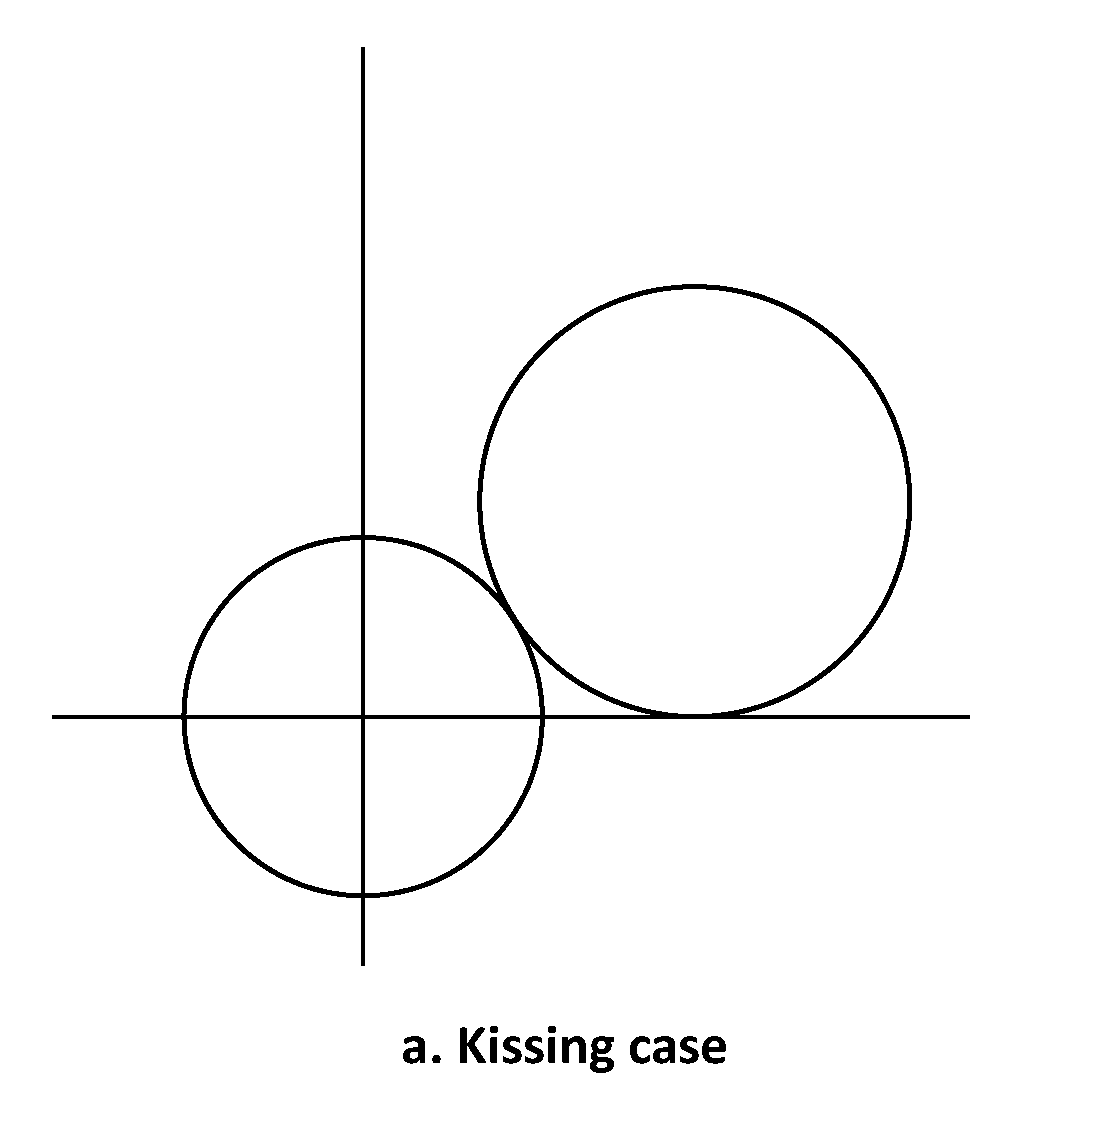
\includegraphics[height=1.65in,width=1.7in]{kissing.eps} &
\includegraphics[height=1.65in,width=1.7in]{convergence.eps}
\end{tabular}
\caption{Limitations for proving UNSAT} 
\label{fig:limit} 
%\end{minipage}
\end{figure} 



\subsection{raSAT loop}

Although an $O.T$ refinement loop is enough to implement an ICP based SMT solver, 
we extend it as {\bf raSAT} (SAT by refinement of approximations) loop to accelerate SAT detection 
by adding $U.T$, which works as in Fig.~\ref{fig:OTrefine}~(b). 
\begin{enumerate}
\item When an over-approximation theory $O.T$ detects $O.T$-UNSAT (resp. $O.T$-valid), 
answer UNSAT (resp. SAT). 
\item When an under-approximation theory $U.T$ detects $U.T$-SAT, answer SAT. 
\item If neither holds, a refinement is applied. 
\end{enumerate}

Our design of an SMT solver {\bf raSAT} applies two heuristic features. 
\begin{itemize}
\item Incremental widening intervals, and incremental deeping search 
(Section~\ref{sec:incsearch}). 
\item 
Heurstic measures {\em SAT-likelyhood} and {\em sensitivity}, 
for selection of a variable to decompose and a box to explore. 
(Section~\ref{sec:SATheuristics}). 
\end{itemize} 

{\bf raSAT} also prepares various interval arithmetic as $O.T$ as in Section~\ref{sec:approximation}, 
whereas currently only random tesing (\emph{k-random ticks}, 
which consists of periodical $k$-test instances with a random offset) is prepared as $U.T$. 

A typical theory for $O.T$ and $U.T$ are an interval arithmetic and testing, respectively. 
We say {\em IA-valid}, {\em IA-SAT}, and {\em IA-UNSAT}, when it is $O.T$-valid, $O.T$-SAT, and 
$O.T$-UNSAT, respectively. 
Similarly, we say {\em test-SAT} and {\em test-UNSAT}, when it is $U.T$-SAT and $U.T$-UNSAT, respectively. 
Note that either IA-valid or test-SAT implies SAT, and IA-UNSAT implies UNSAT, 
whereas IA-SAT and test-UNSAT can conclude neither. 


%We instantiate testing to $U.T$ in Section~\ref{sec:raSATloop}. 
%%%%%%%%%%%%%%%%
\suppress{
\begin{definition}\label{def:testing}
%For $\exists x_1 \in (a_1,b_1) \cdots x_n \in (a_n,b_n). \bigwedge \limits_{i=1}^m f_i(x_1,\cdots,x_n) > 0$, 
Let $M = \bigwedge \limits_{i=1}^m x_i \in (a_i,b_i)$ and 
${\mathcal P} = \bigwedge \limits_{i=1}^m f_i(x_1,\cdots,x_n) > 0$. 
%
Let a choice function $\theta : (\Real \times \Real)^n \rightarrow \Real^n$ 
such that $\theta(M) \in (a_1,b_1) \times \cdots \times (a_n,b_n)$. 
Testing is a finite set $\Theta$ of choice functions. Then, we say 
\begin{itemize}
\item ${\mathcal P}$ is \emph{Test-SAT} under $M$ if $\theta(M)$ holds ${\mathcal P}$ 
for some $\theta \in \Theta$, and 
\item ${\mathcal P}$ is \emph{Test-UNSAT} under $M$ if $\theta(M)$ never holds ${\mathcal P}$ 
for each $\theta \in \Theta$. 
\end{itemize} 
%We denote $I \models_{test(\theta)} P$ if $\bigwedge \limits_{i=1}^m f_i(\theta(I)) > 0$ holds.
\end{definition}
}
%%%%%%%%%%%%%%%%


{\bf raSAT} prepares various Affine intervals, adding to classical interval (CI)~\cite{moore}, 
which keep lower and upper bounds. The weakness of CI is loss of dependency 
among values. For instance, $x - x$ is evaluated to $(-2,2)$ for $x \in (2,4)$. 

Affine Interval~\cite{af,comba93} introduces \emph{noise symbols} $\epsilon$, 
which are interpreted as values in $(-1,1)$. 
For instance, $x = 3 + \epsilon$ describes $x \in (2,4)$, and 
$x - x = (3 + \epsilon) - (3 + \epsilon)$ is evaluated to $0$. 
The drawback is that the multiplication without dependency might be less precise than CI.
Affine intervals also cannot represent infinite intervals, e.g., $(0,\infty)$, 
since it becomes $\infty + \infty~\epsilon$. 
Forms of affine intervals vary by choices how to approximate multiplications. They are,
\begin{enumerate}[(i)]
\item $\epsilon \epsilon'$ is replaced with a fresh noise symbol 
($AF$)~\cite{StolfiThesis,comba93}, 
\item $\epsilon \epsilon'$ is reduced to the fixed error noise symbol 
$\epsilon_{\pm}$ ($AF_1$ and $AF_2$) \cite{af},
\item $\epsilon \epsilon'$ is replaced with $(-1,1) \epsilon$ 
(or $(-1,1) \epsilon'$) ($EAI$)~\cite{ngocsefm},
\item $\epsilon \epsilon$ is reduced to fixed noise symbols 
$\epsilon_+$ or $\epsilon_{-}$ ($AF_2$) \cite{af}, 
\item Chebyshev approximation of $x^2$ introduces a noise symbol $|\epsilon|$ 
as an absolute value of $\epsilon$ with 
$\epsilon \epsilon = |\epsilon| |\epsilon| = |\epsilon| + (-\frac{1}{4}, 0)$ and
$\epsilon |\epsilon| = \epsilon + (-\frac{1}{4}, \frac{1}{4})$ \cite{tapas12}. 
%(Fig.~\ref{fig:chevabs}). 
%\item keeping products of noise symbols up to degree $2$ ($\epsilon_i \epsilon_j$),
\end{enumerate} 

%%%%%%%%%%%%%%%%%
\suppress{
\begin{remark}
For Affine intervals, \emph{sensitivity}~\cite{ngocsefm} of a variable
is a possible range of the absolute value of the coefficient of its corresponding $\epsilon$. 

%In Example~\ref{examp:sensitivity}, $CAI$ estimates the coefficient of $|\epsilon_1|$ as $\textbf{3}$, 
%which has the largest sensitivity and indicates $x$ the most influencial. 

Note that Affine interval works only for bounded intervals. 
For instance, $\infty + \infty \epsilon$ represents $(-\infty,\infty)$, which says nothing. 
Narrowing intervals as an incremental search (Section~\ref{sec:incsearch}) partilly depends on this fact. 
That is, if $\pm \infty$ is contained in an interval, first give finite upper/lower bounds and search 
within these bounds using an Affine interval. If UNSAT is concluded, then enlarge to the whole intervals 
using CI. 
\end{remark}
}
%%%%%%%%%%%%%%%%%


\begin{example} \label{examp:sensitivity}
Let $f = x^3 - 2xy$ with $x = (0,2)$ ($x = 1 + \epsilon_1$) and $y=(1,3)$ ($y = 2+\epsilon_2$), 
we have,
\begin{itemize}
\item $AF_2$ estimates the range of $f$ as 
$-3 - \epsilon_1 - 2\epsilon_2 + 3\epsilon_+ + 3\epsilon_{\pm}$, thus $(-9,6)$,
\item $CAI$ estimates the range of $f$ as 
$(-4,-\frac{11}{4}) + (-\frac{1}{4}, 0)\epsilon_1 - 2\epsilon_2 + \textbf{3}|\epsilon_1| + (-2,2)\epsilon_{\pm}$, 
thus $(-8,4.5)$.
\end{itemize}
\end{example}



%%%%%%%%%%%%%%%%%%%%%%%%%%
\suppress{
\begin{figure}[ht]
\begin{minipage}[b]{1.0\linewidth}
\centering
\begin{tabular}{ll}
\includegraphics[height=1.6in,width=1.7in]{chev1.pdf} &
\includegraphics[height=1.6in,width=1.7in]{chev2.pdf}
\end{tabular}
\caption{Chebyshev approximation of $x^2$ and $x~|x|$}
\label{fig:chevabs}
\end{minipage}
\end{figure}

$CAI$ \cite{tapas12} consists of (ii) and (v), which keeps better precision than iv)
for multiplicatins of the same variables, e.g., Taylor expansion. 
%To improve precision in estimating upper and lower bounds of polynomials, we apply 
%\textbf{Affine Arithmetic} such as $AF_1$, $AF_2$ \cite{af}, $CAI$ ~\cite{tapas12} 
%instead of Classical Interval \cite{moore}. 
%Note that upper and lower bounds estimated by IA are over-approximation bounds of polynomials.

}
%%%%%%%%%%%%%%%%%%%%%%%%%%
\suppress{
\begin{definition}
%For $\exists x_1 \in (a_1,b_1) \cdots x_n \in (a_n,b_n). \bigwedge \limits_{i=1}^m f_i(x_1,\cdots,x_n) > 0$, 
Let $M = \bigwedge \limits_{i=1}^m x_i \in (a_i,b_i)$ and 
${\mathcal P} = \bigwedge \limits_{i=1}^m f_i(x_1,\cdots,x_n) > 0$. 
%
Let $\delta_i^l$ and $\delta_i^u$ be lower and upper bounds of $f_i(x_1,\cdots,x_n)$ 
estimated by IA for $x_i \in (a_i,b_i)$. Then, we say 
%
%\vspace*{0.5em}
\begin{itemize}
\item ${\mathcal P}$ is \emph{IA-VALID} under $M$, if IA evaluates 
$~\forall i \in [1,m].~\delta_i^l > 0$,
%\vspace*{0.33em}
\item ${\mathcal P}$ is \emph{IA-UNSAT} under $M$, 
$~\exists i \in [1,m].~\delta_i^u \leq 0$, and 
\item ${\mathcal P}$ is \emph{IA-SAT} under $M$, if 
$(\exists j \in [1,m].~\delta_j^l \leq 0)\; \wedge \; 
	(\bigwedge \limits_{i=1}^m \delta_i^u > 0)$.
\end{itemize} 
\end{definition}

IA-VALID and IA-UNSAT safely reason satisfiability (SAT) and unsatisfiability (UNSAT), 
respectively. However, IA-SAT cannot conclude SAT. 
}


\include{refinement-strategies}

\chapter{Equality handling}
\subsection{Greater-than-or-Equal Handling} \label{sec:geq}

{\bf raSAT} loop is designed to solve polynomial inequality. 
There are several ways to extend to handle equality, in which our idea shares similarity with 
dReal~\cite{dRealCADE13,dRealLICS12}. 

\begin{definition} \label{def:strict_unsat}
$\bigwedge \limits_{j} f_j \geq 0$ is 
{\em strict-SAT} (resp. {\em strict-UNSAT}) 
if $\bigwedge \limits_{j} f_j > \delta_j$ is SAT 
(resp. $\bigwedge \limits_{j} f_j > -\delta_j$ is UNSAT) for some $\delta_j >0$.
\end{definition}

\begin{lemma} \label{lem:strict_sat}
If $\bigwedge \limits_{j} f_j \geq 0$ is {\em strict-SAT} (resp. {\em strict-UNSAT}), 
it is SAT (resp. UNSAT).
\end{lemma}

Note that netiher strict-SAT nor strict-UNSAT (i.e., kissing situation), 
%if $\bigwedge \limits_{j} f_j \geq 0$ is SAT but $\bigwedge \limits_{j} f_j > 0$ is UNSAT 
Lemma~\ref{lem:strict_sat} cannot conclude anything, and \textbf{raSAT} says {\em unknown}. 
%In implementation of \textbf{raSAT}, when $\geq$ appears, exploration of IA-SAT 
%(resp. IA-UNSAT) is reduced to that of IA-strict-SAT (resp. IA-strict-UNSAT). 


\subsection{SAT on Equality by Intermediate Value Theorem} \label{sec:eq}
For solving polynomial constraints with single equality ($g=0$), we apply {\em Intermediate Value Theorem}. 
That is, if existing 2 test cases such that $g > 0$ and $g < 0$, then $g=0$ is SAT somewhere in between, 
as in Fig.~\ref{fig:ivt}. 

\begin{lemma} \label{lemma:ivt}
For $F = \exists x_1 \in (a_1,b_1) \wedge \cdots \wedge x_n \in (a_n,b_n). 
\bigwedge \limits_{j}^m f_j > 0~\wedge~g = 0$, $F$ is SAT, if 
there is a box $(l_1, h_1) \times \cdots \times (l_n,h_n)$ with $ (l_i,h_i) \subseteq (a_i,b_i)$ 
such that 
\begin{enumerate}[(i)]
\item $\bigwedge \limits_{j}^m f_j > 0$ is IA-VALID in the box, and 
\item there are two instances $\vec{t},\vec{t'}$ in the box with $g(\vec{t}) > 0$ and $g(\vec{t'}) < 0$.
\end{enumerate}
\end{lemma}

{\bf raSAT} first tries to find an IA-VALID box for $\bigwedge \limits_{j}^m f_j > 0$ by refinements. 
If such a box is found, it tries to find 2 instances for $g > 0$ and $g < 0$ by testing. 
Intermediate Value Theorem guarantees the existence of an SAT instance in between. 
Note that this method works for single equality and does not find an exact SAT instance. 
If multiple equalities do not share variables each other, we can apply Intermediate Value Theorem 
repeatedly to decide SAT. In Zankl benchmarks in SMT-lib, there are 15 gen-**.smt2 that contain equality
(among 166 problems), and each of them satisty this condition. 


 
\suppress{
In Table \ref{tab:eqexp} we show preliminary experiment for 15 problems that contain polynomial equalities in Zankl family. \textbf{raSAT} works well for these SAT problems and it can detect all SAT problems (11 among 15). At the current implementation, raSAT reports \emph{unknown} for UNSAT problems. The first 4 columns indicate \emph{name of problems}, \emph{the number of variables}, \emph{the number of polynomial equalities} and \emph{the number of inequalities}  in each problem, respectively. The last 2 columns show comparison results of \textbf{Z3 4.3} and \textbf{raSAT}.
\begin{table}
\centering
\scalebox{1.0}{
\begin{tabular}[b]{|c|c|c|c|c|c|c|c|}
\hline
%\multirow{2}{*}{Problem} & {No.} & {No.} & {No.}&
{Problem} & {No.} & {No.} & {No.}&
\multicolumn{2}{c|}{\textbf{Z3 4.3} (15/15)} &\multicolumn{2}{c|}{\textbf{raSAT} (11/15)}\\
\cline{5-8}
Name & Variables& Equalities& Inequalities&{Result} & {Time(s)}&{Result} & {Time(s)}\\
\hline
gen-03 & 1 & 1 & 0& SAT &0.01 & SAT &0.015\\
\hline
gen-04 & 1 & 1 & 0& SAT &0.01 & SAT &0.015\\
\hline
gen-05 & 2 & 2 & 0& SAT &0.01 & SAT &0.046\\
\hline
gen-06 & 2 & 2 & 1& SAT &0.01 & SAT &0.062\\
\hline
gen-07 & 2 & 2 & 0& SAT &0.01 & SAT &0.062\\
\hline
gen-08 & 2 & 2 & 1& SAT &0.01 & SAT &0.062\\
\hline
gen-09 & 2 & 2 & 1& SAT &0.03 & SAT &0.062\\
\hline
gen-10 & 1 & 1 & 0& SAT &0.02 & SAT &0.031\\
\hline
gen-13 & 1 & 1 & 0& UNSAT &0.05 & unknown &0.015\\
\hline
gen-14 & 1 & 1 & 0& UNSAT &0.01 & unknown &0.015\\
\hline
gen-15 & 2 & 3 & 0& UNSAT &0.01 & unknown &0.015\\
\hline
gen-16 & 2 & 2 & 1& SAT &0.01 & SAT &0.062\\
\hline
gen-17 & 2 & 3 & 0& UNSAT &0.01 & unknown &0.031\\
\hline
gen-18 & 2 & 2 & 1& SAT &0.01 & SAT &0.078\\
\hline
gen-19 & 2 & 2 & 1& SAT &0.05 & SAT &0.046\\
\hline
\end{tabular}
}
\caption{Experimental results for 15 equality problems of Zankl family}
\label{tab:eqexp}
\end{table}

We also apply the same idea for multiple equalities $\bigwedge \limits_{i} g_i = 0$ such that $Var(g_k) \cap Var(g_{k'}) = \emptyset$ where $Var(g_k)$ is denoted for the set of variables in the polynomial $g_k$. In the next section we will present idea for solving general cases of multiple equalities.
}

}
%%%%%%%%%%%%%%%%%%%%%%%%%%%%%


\chapter{SMT solver design}
We design an SMT solver named raSAT~\footnote{\url{http://www.jaist.ac.jp/~mizuhito/tools/rasat.html}} to solve polynomial constraint. 


\begin{figure}[ht]
%\begin{minipage}[b]{1.0\linewidth}
\centering
\includegraphics[width=\textwidth]{smt-design.png} 
\caption{raSAT design} 
\label{fig:smt-design} 
%\end{minipage}
\end{figure} 

\chapter{Experiments}
This chapter is going to present the experiments results which reflect how effective our designed strategies are. In addition, comparison between raSAT, Z3 and iSAT3 will be also shown. The experiments were done on a system with  Intel Xeon E5-2680v2 2.80GHz and 4 GB of RAM. In the experiments, we exclude the problems which contain equalities because currently raSAT focuses on inequalities only.

\section{Experiments on Strategy Combinations} \label{sec:expstrategy}

We perform experiments only on Zankl, and Meti-Tarski families. 


Our combinations of strategies mentioned in Section~\ref{sec:SATheuristics} are, 

\medskip
{\centering
\begin{tabular}{l|l|l}
Selecting a test-UNSAT API~~ & Selecting a box (to explore): & 
Selcting a variable: \\  % (for testing and decomposition)
\hline

(1) Least SAT-likelyhood. & 
(3) Largest number of SAT inequalities.~~ & 
(8) Largest sensitibity. \\

(2) Largest SAT-likelyhood. & 
(4) Least number of SAT inequalities. & \\

& (5) Largest SAT-likelyhood. & \\

& (6) Least SAT-likelyhood. & \\

(10) Random. & (7) Random. & (9) Random. \\
\end{tabular}
}
\medskip

Table~\ref{tab:rasat-experiments} shows the experimental results of above mentioned combination. 
The timeout is set to 500s, and each time is the total of successful cases 
(either SAT or UNSAT). 

Note that (10)-(7)-(9) means all random selection. 
Generally, the combination of (5) and (8) show the best results, 
though the choice of (1),(2), and (10) shows different behavior on benchmarks. 
We tentatively prefer (1) or (10), but it needs to be investigated further. 

\begin{table*}[t]
\centering
\resizebox{\columnwidth}{!}{%
\begin{tabular}{ | l | r | r  r | r | r  | r | r | r | r | r | r |r | r |}
\hline
    \multicolumn{1}{|l|}{Benchmark} & 
    \multicolumn{3}{c|}{(1)-(5)-(8)} & \multicolumn{2}{c|}{(1)-(5)-(9)} & 
    \multicolumn{2}{c|}{(1)-(6)-(8)} & \multicolumn{2}{c|}{(1)-(6)-(9)} &
    \multicolumn{2}{c|}{(10)-(5)-(8)} & \multicolumn{2}{c|}{(10)-(6)-(8)} 
\\
\hline
 Matrix-1 (SAT) & 20 & 132.72 & (s) & 21 & 21.48 & 19 & 526.76 & 18 & 562.19 & 21 & 462.57 & 19 & 155.77 
\\
\hline
 Matrix-1 (UNSAT) & 2 & 0.00 && {\bf 3} & 0.00 & {\bf 3} & 0.00 & {\bf 3} & 0 & {\bf 3} & 0.00 
& {\bf 3} & 0.00 
\\
\hline
 Matrix-2,3,4,5 (SAT) & {\bf 11} & 632.37 && 1 & 4.83 & 0 & 0.00 & 1 & 22.50 & 9 & 943.08 & 1 & 30.48 
\\
\hline
 Matrix-2,3,4,5 (UNSAT) & 8 & 0.37 && 8 & 0.39 & 8 & 0.37 & 8 & 0.38 & 8 & 0.38 & 8 & 0.38 
\\
\hline
\hline
    \multicolumn{1}{|l|}{Benchmark} & 
    \multicolumn{3}{c|}{(2)-(5)-(8)} & \multicolumn{2}{c|}{(2)-(5)-(9)} & 
    \multicolumn{2}{c|}{(2)-(6)-(8)} & \multicolumn{2}{c|}{(2)-(6)-(9)} & 
    \multicolumn{2}{c|}{(2)-(7)-(8)} & \multicolumn{2}{c|}{(10)-(7)-(9)} \\
\hline
 Matrix-1 (SAT) & {\bf 22} & 163.47 & (s) & 19 & 736.17 & 20 & 324.97 & 18 & 
1068.40 & 21 & 799.79 & 21 & 933.39 
\\
\hline
 Matrix-1 (UNSAT) &     2 & 0 && 2 & 0.00 & 2 & 0.00 & 2 & 0.00 & 2 & 0.00 & 2 & 0.00 
\\
\hline
 Matrix-2,3,4,5 (SAT) &     5 & 202.37 && 1 & 350.84 & 1 & 138.86 & 0 & 0.00 & 0 & 0.00 & 0 & 0.00 
\\
\hline
 Matrix-2,3,4,5 (UNSAT) &     8 & 0.43 && 8 & 0.37 & 8 & 0.40 & 8 & 0.38 & 8 & 0.37 & 8 & 0.38 
\\
\hline
\hline
    \multicolumn{1}{|l|}{Benchmark} & 
    \multicolumn{3}{c|}{(1)-(3)-(8)} & \multicolumn{2}{c|}{(1)-(4)-(8)} & 
    \multicolumn{2}{c|}{(2)-(3)-(8)} & \multicolumn{2}{c|}{(2)-(4)-(8)} & 
    \multicolumn{2}{c|}{(10)-(3)-(8)} & \multicolumn{2}{c|}{(10)-(4)-(8)} \\
\hline
 Matrix-1 (SAT) & 20 & 738.26 & (s) & 21 & 1537.9 & 18 & 479.60 & 21 & 867.99 & 20 & 588.78 & 19 & 196.21 
\\
\hline
 Matrix-1 (UNSAT) & 2 & 0.00 && 2 & 0.00 & 2 & 0.00 & 2 & 0.00 & 2 & 0.00 & 2 & 0.00 
\\
\hline
 Matrix-2,3,4,5 (SAT) & 0 & 0.00 && 2 & 289.17 & 1 & 467.12 & 1 & 328.03 & 1 & 195.18 & 2 & 354.94 
\\
\hline
 Matrix-2,3,4,5 (UNSAT) & 8 & 0.36 && 8 & 0.36 & 8 & 0.34 & 8 & 0.37 & 8 & 0.37 & 8 & 0.39 
\\
\hline
\end{tabular}
}
\bigskip
\resizebox{\columnwidth}{!}{%
\begin{tabular}{ | l | r | r  r | r  | r | r | r | r | r |}
\hline
    \multicolumn{1}{|l|}{Benchmark} & 
    \multicolumn{3}{c|}{(1)-(5)-(8)} & \multicolumn{2}{c|}{(1)-(5)-(9)} & 
    \multicolumn{2}{c|}{(10)-(5)-(8)} & \multicolumn{2}{c|}{(10)-(7)-(9)} \\
\hline
    Meti-Tarski (SAT, 3528) & 3322 & 369.60 & (s) & 3303 & 425.37 & {\bf 3325} & 653.87 & 3322 & 642.04 
\\
\hline
    Meti-Tarski (UNSAT, 1573) & 1052 & 383.40 && 1064 & 1141.67 & {\bf 1100} & 842.73 & 1076 & 829.43 
\\
\hline
\end{tabular}
}
\medskip
\caption{Combinations of {\bf raSAT} strategies on NRA/Zankl,Meti-Tarski benchmark} 
\label{tab:rasat-experiments}
\end{table*}


\section{Comparison with other SMT Solvers}

We compare {\bf raSAT} with other SMT solvers on NRA benchmarks, Zankl and Meti-Tarski. 
The timeouts for Zankl and Meti-tarski are $500s$ and $60s$, respectively. 
For {\bf iSAT3}, ranges of all variables are uniformly set to be in the range $[-1000, 1000]$
(otherwise, it often causes segmentation fault). 
Thus, UNSAT detection of {\bf iSAT3} means UNSAT in the range $[-1000, 1000]$, 
while that of {\bf raSAT} and {\bf Z3 4.3} means  UNSAT over $[-\infty, \infty]$. 

Among these SMT solvers, {\bf Z3 4.3} shows the best performance. 
However, if we closely observe, there are certain tendency. 
{\bf Z3 4.3} is very quick for small constraints, i.e., with 
short APIs (up to $5$) and a small number of variables (up to $10$). 
{\bf raSAT} shows comparable performance on SAT detection with 
longer APIs (larger than $5$) and a larger number of variables (more than $10$), 
and sometimes outforms for SAT detection on vary long constraints 
(APIs longer than $40$ and/or more than $20$ variables). 
Such examples appear in Zankl/matrix-3-all-*, matrix-4-all-*, and matrix-5-all-* 
(total 74 problems), and {\bf raSAT} solely solves 
\begin{itemize}
\item[$\bullet$] {\em matrix-3-all-2} (47 variables, 87 APIs, and max length of an API is 27), 
\item[$\bullet$] {\em matrix-3-all-5} (81 variables, 142 APIs, and max length of an API is 20), 
\item[$\bullet$] {\em matrix-4-all-3} (139 variables, 244 APIs, and max length of an API is 73), and 
\item[$\bullet$] {\em matrix-5-all-01} (132 variables, 276 APIs, and max length of an API is 47). 
\end{itemize}
Note that, for Zankl, when UNSAT is detected, it is detected very quickly. 
This is because SMT solvers detects UNSAT only when they find small UNSAT cores, 
without tracing all APIs. However, for SAT detection with ;arge problems, 
SMT solvers need to trace all problems. Thus, it takes much longer time. 

\begin{table*}[t]
\centering
\resizebox{\columnwidth}{!}{%
\begin{tabular}{ | l | r | r  r | r | r  | r | r | r | r | r | r |r | r |}
\hline
    \multicolumn{1}{|l|}{Benchmark} & 
    \multicolumn{5}{c|}{\bf raSAT} & \multicolumn{4}{c|}{\bf Z3 4.3} & \multicolumn{4}{c|}{\bf iSAT3} \\
\hline
    & \multicolumn{3}{|c|}{SAT} & \multicolumn{2}{|c|}{UNSAT} & \multicolumn{2}{|c|}{SAT} 
    & \multicolumn{2}{|c|}{UNSAT} & \multicolumn{2}{|c|}{SAT} & \multicolumn{2}{|c|}{UNSAT} \\
\hline
Zankl/matrix-1 (53) & 20 & 132.72 & (s) & 2 & 0.00 & 41 & 2.17 & 12 & 0.00 & 11 & 4.68 & 3 & 0.00 \\
\hline
Zankl/matrix-2,3,4,5 (98) & 11 & 632.37 && 8 & 0.37 & 13 & 1031.68 & 11 & 0.57 & 3 & 196.40 & 12 & 8.06 \\
\hline 
Meti-Tarski (3528/1573) & 3322 & 369.60 && 1052 & 383.40 & 3528 & 51.22 & 1568 & 78.56 & 2916 & 811.53 & 
1225 & 73.83 \\
\hline
\end{tabular}
}
\medskip 
\caption{Comparison among SMT solvers} \label{tab:comparison}
\end{table*}


\section{Experiments with QE-CAD Benchmark}
We also did experiments on QE-CAD problems provided by Mohab Safey El Din\footnote{\url{http://www-polsys.lip6.fr/~safey/}} - LIP6 who is working on QE-CAD simplification (checking SAT/UNSAT only and the complexity is from DEXP to EXP) and the QEPCAD problems collected by Hidenao Iwane\footnote{\url{https://github.com/hiwane/qepcad/}}. 

The benchmarks from LIP6 are all unsatisfiable and contain long polynomials (in terms of monomials number). From the experiments with raSAT and Z3, these benchmarks show that they are very difficult to be solved (Table~\ref{exp:lip6}). These benchmarks may be suitable targets for our UNSAT core strategies in the future. 

\begin{table} \label{exp:hiwane}
\begin{center}
\begin{tabular}{|c|c|c|c|c|c|c|c|}
\hline
\multicolumn{4}{|c|}{raSAT} & \multicolumn{4}{c|}{Z3}\\ \hline
\multicolumn{2}{|c|}{SAT}  & \multicolumn{2}{c|}{UNSAT} & \multicolumn{2}{c|}{SAT} & \multicolumn{2}{c|}{UNSAT} \\ \hline
156 & 244.6(s) & 2 & 0.03 (s) & 205 & 1.12 (s) & 22 & 0.05 (s) \\ \hline
\end{tabular}
\end{center}
\caption{Experiments on 217 QEPCAD problems from Hidenao Iwane}
\end{table}

In terms of QEPCAD benchmarks, while Z3 solves all $217$ problems, raSAT solves $156/205$ satisfiable and $2/22$ unsatisfiable benchmarks. Apart from a number of problems which raSAT has errors in parsing, the unsolved ones are mostly unsatisfiable. This can be tackled by strategies on UNSAT core which is left for our future works. 
\begin{table} \label{exp:lip6}
\begin{center}
\begin{tabular}{| c | c | c | c | c |}
\hline
\multirow{2}{*}{Problem} & \multicolumn{2}{ c }{raSAT} & \multicolumn{2}{ |c| }{Z3}\\ \cline{2-5}& Time (s) & Result & Time (s) & Result\\ \hline
f23 & 3600 & Timeout & 3599.55 & Timeout\\ \hline
f22 & 3600 & Timeout & 3599.51 & Timeout\\ \hline
pol & 3600 & Timeout & 0.02499 & UNSAT\\ \hline
f13 & 3600 & Timeout & 3599.17 & Timeout\\ \hline
pol1 & 3600 & Timeout & 3601.61 & Timeout\\ \hline
f12 & 3600 & Timeout & 3599.27 & Timeout\\ \hline
\end{tabular}
\caption{Experiments on problems from LIP6}
\end{center}
\end{table}


%%%%%%%%%%%%%%%%%

\chapter{Conclusion}


This thesis presented improvement and extensions for an SMT solved {\bf raSAT} including heuristics to deal with exponential exploration of boxes, extensions for handling equations and handling constraints over integer numbers.

\section*{Observation and Discussion} 

From experimental results in Section~\ref{sec:experiments} and~\ref{sec:expsmtlib}, 
we observe the followings. 
\begin{itemize}
\item The degree of polynomials will not affect much. 
\item The number of variables are matters, but also for Z3 4.3. 
The experimental results do not show exponential growth, and we expect 
the strategy of selection of an API in which related intervals are decomposed
seems effective in practice. By observing Zankl examples, we think the maximum 
number of variables of each API seems a dominant factor. 
\item Effects of the number of APIs are not clear at the moment. In simple benchmarks, 
{\bf raSAT} is faster than Z3 4.3, however we admit that we have set small degree $n=6$
for each API. 
\end{itemize}

For instance, {\em matrix-2-all-5,8,11,12} in Zankl 
contain a long monomial (e.g., $60$) with the max degree $6$, and 
relatively many variables (e.g., $14$), which cannot be solved by Z3 4.3, but 
{\bf raSAT} does. 
As a general feeling, if an API contains more than $30 \sim 40$ variables, 
{\bf raSAT} seems saturating. 
We expect that, adding to a strategy to select an API (Section~\ref{sec:intervaldecomp}), 
we need a strategy to select variables in the focus. We expect this can be designed 
with sensitivity (Example~\ref{examp:sensitivity}) and would work in practice. 
Note that sensitivity can be used only with noise symbols in Affine intervals. 
Thus, iSAT and RSOLVER cannot use this strategy, though they are based on IA, too. 

\section*{Future Work}

\medskip \noindent 
{\bf UNSAT core}

\medskip \noindent 
{\bf Exact confirmation}.
Currently, {\bf raSAT} uses iRRAM to verify SAT instances only. 
We are planning to implement confirmation phase to UNSAT cases. 

\medskip \noindent 
{\bf Further strategy refinement}. 
Test data generation, blanced box decomposition


%%%
\suppress{
\subsubsection{Extension of {\bf raSAT} loop}
\begin{itemize}
\item {\bf Equality handling}: currently, {\bf raSAT} loop can handle only inequalities. 
Before applying ideal based technique, such as {\em Gr{\"o}bner basis}, 
we are planning to implement a non-constructive detection of equality 
by {\em intermediate value theorem}. 

\suppress{
\item{\textbf{Polynomial equality by Intermediate value theorem}:} 
Consider 
\begin{center}
$(x_1 \in (a_1,b_1) \wedge \cdots \wedge x_n \in (a_n,b_n))~\bigwedge 
\limits_{j}^m f_j(x_1,\cdots,x_n) > 0~\wedge~g(x_1,\cdots, x_n) = 0.$
\end{center}
SAT can be proved by two steps. First, find a box of the product of 
$(l_{ik},h_{ik}) \subseteq (l_i,h_i)$ (by interval arithmetic) such that 
\begin{center}
$\forall x_1 \in (l_{1k},h_{1k}) \cdots x_n \in (l_{nk},h_{nk}).~\bigwedge 
 \limits_{j}^m f_j(x_1,\cdots,x_n) > 0$~~~~(IA-VALID) 
\end{center}
and find two instances (by testing) in the box with $g(a_1,\cdots,a_n) > 0$ 
and $g(b_1,\cdots,b_n) < 0$. By Intermediate value theorem, we can conclude 
$\exists x_1 \in (l_1,h_1) \cdots x_n \in (l_n,h_n).~g(x_1,\cdots, x_n) = 0$. 
}

\item \textbf{Solving polynomial constraints on integers}: 
In integer domain, the number of test data is finite if interval constraints are bounded. 
Then, Test-UNSAT implies UNSAT if all possible test data are generated. 
A tight interaction between testing and interval decomposition could be investigated.
Mixed integers are also challenging. 
\end{itemize}


\subsubsection{\textbf{raSAT} Development}

\begin{itemize}
\item \textbf{Avoiding local optimal}: 
we borrow an idea of \emph{restart} in MiniSAT for escaping from hopeless local search 
(i.e., solution set is not dense or empty). 
\emph{Heuristics} would be, after a deep interval decomposition of 
a box and Test-UNSAT are reported, backtrack occurs to choose a randomly selected box. 

\item \textbf{Separation of linear constraints}: 
Many benchmarks contain linear constraints. Current implementation does not have 
any tuning, but {\bf raSAT} loop only. 
Practically, separating linear and non-linear constraints and solving them 
in a coordinated way between Presbuger arithmetic and {\bf raSAT} would improve. 
During this separation, variables of intersecting linear constraints would be candidates 
for interval decompositions. 

\item \textbf{Incremental DPLL}: For interactions with the SAT solver, 
we currently apply the very lazy theory learning. Combination with 
\emph{eager} theory propagation would improve, in which we can propagate 
a conflict from a partial truth assignment instead of waiting 
for a full truth assignment obtained by SAT solver.
\end{itemize}
}
%%

%%
\suppress{
\subsection{Applications}
\begin{itemize}
\item \textbf{Checking overflow and roundoff error}: In the computers, the real numbers are represented by finite numbers (i.e., floating point numbers, fixed point numbers). Due to finite representation, the over-flow and roundoff errors (OREs) \cite{ngocsefm, ngocase} may occur. The OREs will be propagated through computations of the program. Further, the computations themselves also cause OREs because the arithmetic needs to round the result to fit the number format. Besides, OREs are also affected by types of statements, i.e., branch, loop, assignment statements.
By symbolic execution, ORE constraints are propagated from a program and ORE problems are reduced to problems of solving ORE constraints for verifying whether OREs occur. 
%For solving ORE constraint, combination of the new form of affine arithmetic ($CAI_1$) and \emph{sensitivity} (i.e., high degrees, )

\item \textbf{Loop invariant generation}: The problem of linear invariant generation is often reduced to the problem of non-linear constraint solving. 
Since Farkas's Lemma \cite{Colon03} uses the product of matrices with polynomial constraint solving, we can extend the target for non-linear invariant generation.
%Based on Farkas' Lemma \cite{Colon03}, non-linear constraints on coefficients of the target linear invariant are generated and a satisfiable instance of these constraints is a candidate of the linear invariant. 
\end{itemize}
}
%%

\end{document}
